\chapter{Numerische Tests}
\label{cha:NumerischeTests}

In diesem Kapitel möchten wir die vorgestellten Verfahren verschiedenen numerischen Tests unterziehen. Dabei wollen wir hauptsächlich den Fehler der numerischen Lösung zur analytischen untersuchen, aber auch die Kondition der Kollokationsmatrizen, die Parameterwahl und die Laufzeit betrachten. Zusätzlich werden wir die Verfahren mit der finiten Elemente Methode (\acs{FEM}) vergleichen.

Dafür betrachten wir die Poisson-Gleichung mit Dirichlet-Randbedingung auf $\Omega = [-1,1] \times [-1,1] \subset \mathbb{R}^n$:
\begin{align*}
- \Delta u &= 2\pi^2 \sin(\pi x)\sin(\pi y)&&, (x,y) \in \Omega\\
u &= 0&&, (x,y) \in \partial \Omega
\end{align*}
mit analytischer Lösung $u(x,y) = \sin(\pi x)\sin(\pi y)$, dargestellt in Abbildung \ref{fig:plot}. Wir wählen als Gewichtsfunktion $w$ für $\Omega$ die Funktion aus Beispiel \ref{ex:Gewicht}:
\begin{align*}
w = -x^2-y^2+2 - \sqrt{x^4 -2x^2 + y^4 -2y^2+2}.
\end{align*}
\begin{figure}[h]
\centering
\resizebox {\columnwidth} {!} {
% This file was created by matlab2tikz.
%
%The latest updates can be retrieved from
%  http://www.mathworks.com/matlabcentral/fileexchange/22022-matlab2tikz-matlab2tikz
%where you can also make suggestions and rate matlab2tikz.
%
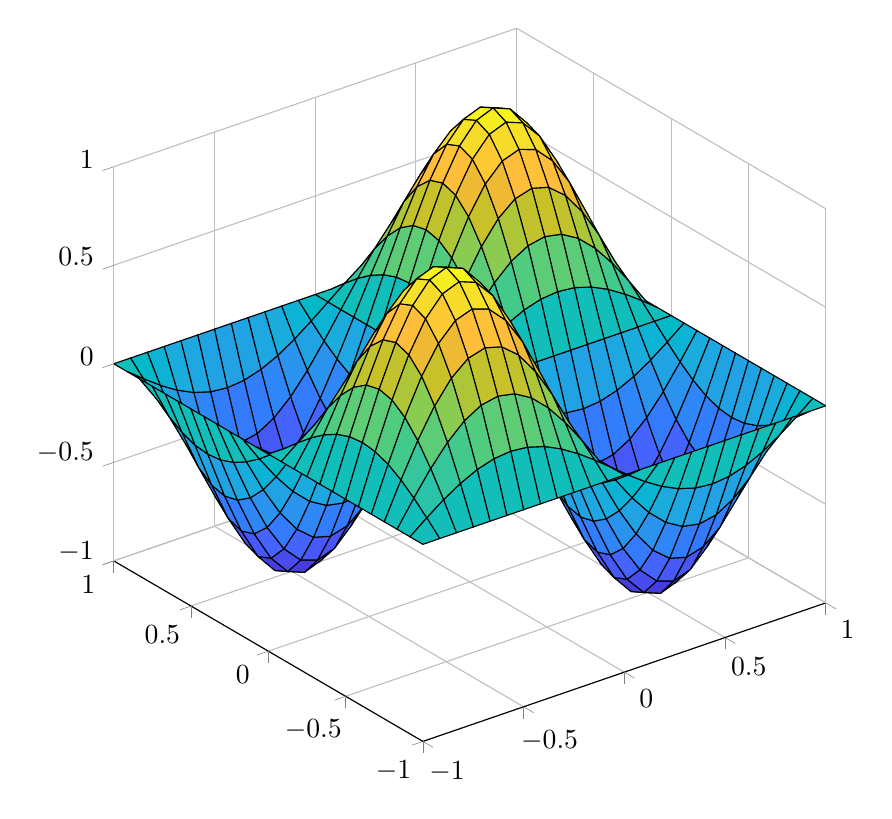
\begin{tikzpicture}

\begin{axis}[%
width=3.56in,
height=3.566in,
at={(0.597in,0.481in)},
scale only axis,
xmin=-1,
xmax=1,
tick align=outside,
ymin=-1,
ymax=1,
zmin=-1,
zmax=1,
view={-37.5}{30},
axis background/.style={fill=white},
axis x line*=bottom,
axis y line*=left,
axis z line*=left,
xmajorgrids,
ymajorgrids,
zmajorgrids,
legend style={at={(1.03,1)}, anchor=north west, legend cell align=left, align=left, draw=white!15!black}
]

\addplot3[%
surf,
shader=flat corner, draw=black, z buffer=sort, colormap={mymap}{[1pt] rgb(0pt)=(0.2422,0.1504,0.6603); rgb(1pt)=(0.25039,0.164995,0.707614); rgb(2pt)=(0.257771,0.181781,0.751138); rgb(3pt)=(0.264729,0.197757,0.795214); rgb(4pt)=(0.270648,0.214676,0.836371); rgb(5pt)=(0.275114,0.234238,0.870986); rgb(6pt)=(0.2783,0.255871,0.899071); rgb(7pt)=(0.280333,0.278233,0.9221); rgb(8pt)=(0.281338,0.300595,0.941376); rgb(9pt)=(0.281014,0.322757,0.957886); rgb(10pt)=(0.279467,0.344671,0.971676); rgb(11pt)=(0.275971,0.366681,0.982905); rgb(12pt)=(0.269914,0.3892,0.9906); rgb(13pt)=(0.260243,0.412329,0.995157); rgb(14pt)=(0.244033,0.435833,0.998833); rgb(15pt)=(0.220643,0.460257,0.997286); rgb(16pt)=(0.196333,0.484719,0.989152); rgb(17pt)=(0.183405,0.507371,0.979795); rgb(18pt)=(0.178643,0.528857,0.968157); rgb(19pt)=(0.176438,0.549905,0.952019); rgb(20pt)=(0.168743,0.570262,0.935871); rgb(21pt)=(0.154,0.5902,0.9218); rgb(22pt)=(0.146029,0.609119,0.907857); rgb(23pt)=(0.138024,0.627629,0.89729); rgb(24pt)=(0.124814,0.645929,0.888343); rgb(25pt)=(0.111252,0.6635,0.876314); rgb(26pt)=(0.0952095,0.679829,0.859781); rgb(27pt)=(0.0688714,0.694771,0.839357); rgb(28pt)=(0.0296667,0.708167,0.816333); rgb(29pt)=(0.00357143,0.720267,0.7917); rgb(30pt)=(0.00665714,0.731214,0.766014); rgb(31pt)=(0.0433286,0.741095,0.73941); rgb(32pt)=(0.0963952,0.75,0.712038); rgb(33pt)=(0.140771,0.7584,0.684157); rgb(34pt)=(0.1717,0.766962,0.655443); rgb(35pt)=(0.193767,0.775767,0.6251); rgb(36pt)=(0.216086,0.7843,0.5923); rgb(37pt)=(0.246957,0.791795,0.556743); rgb(38pt)=(0.290614,0.79729,0.518829); rgb(39pt)=(0.340643,0.8008,0.478857); rgb(40pt)=(0.3909,0.802871,0.435448); rgb(41pt)=(0.445629,0.802419,0.390919); rgb(42pt)=(0.5044,0.7993,0.348); rgb(43pt)=(0.561562,0.794233,0.304481); rgb(44pt)=(0.617395,0.787619,0.261238); rgb(45pt)=(0.671986,0.779271,0.2227); rgb(46pt)=(0.7242,0.769843,0.191029); rgb(47pt)=(0.773833,0.759805,0.16461); rgb(48pt)=(0.820314,0.749814,0.153529); rgb(49pt)=(0.863433,0.7406,0.159633); rgb(50pt)=(0.903543,0.733029,0.177414); rgb(51pt)=(0.939257,0.728786,0.209957); rgb(52pt)=(0.972757,0.729771,0.239443); rgb(53pt)=(0.995648,0.743371,0.237148); rgb(54pt)=(0.996986,0.765857,0.219943); rgb(55pt)=(0.995205,0.789252,0.202762); rgb(56pt)=(0.9892,0.813567,0.188533); rgb(57pt)=(0.978629,0.838629,0.176557); rgb(58pt)=(0.967648,0.8639,0.16429); rgb(59pt)=(0.96101,0.889019,0.153676); rgb(60pt)=(0.959671,0.913457,0.142257); rgb(61pt)=(0.962795,0.937338,0.12651); rgb(62pt)=(0.969114,0.960629,0.106362); rgb(63pt)=(0.9769,0.9839,0.0805)}, mesh/rows=25]
table[row sep=crcr, point meta=\thisrow{c}] {%
%
x	y	z	c\\
-1	-1	1.49975978266186e-32	1.49975978266186e-32\\
-0.916666666666667	-1	0	0\\
-0.833333333333333	-1	6.12323399573676e-17	6.12323399573676e-17\\
-0.75	-1	8.65956056235493e-17	8.65956056235493e-17\\
-0.666666666666667	-1	1.06057523872491e-16	1.06057523872491e-16\\
-0.583333333333333	-1	1.18291797137867e-16	1.18291797137867e-16\\
-0.5	-1	1.22464679914735e-16	1.22464679914735e-16\\
-0.416666666666667	-1	1.18291797137867e-16	1.18291797137867e-16\\
-0.333333333333333	-1	1.06057523872491e-16	1.06057523872491e-16\\
-0.25	-1	8.65956056235493e-17	8.65956056235493e-17\\
-0.166666666666667	-1	6.12323399573676e-17	6.12323399573676e-17\\
-0.0833333333333334	-1	3.16961915143177e-17	3.16961915143177e-17\\
0	-1	-0	-0\\
0.0833333333333333	-1	-3.16961915143176e-17	-3.16961915143176e-17\\
0.166666666666667	-1	-6.12323399573677e-17	-6.12323399573677e-17\\
0.25	-1	-8.65956056235493e-17	-8.65956056235493e-17\\
0.333333333333333	-1	-1.06057523872491e-16	-1.06057523872491e-16\\
0.416666666666667	-1	-1.18291797137867e-16	-1.18291797137867e-16\\
0.5	-1	-1.22464679914735e-16	-1.22464679914735e-16\\
0.583333333333333	-1	-1.18291797137867e-16	-1.18291797137867e-16\\
0.666666666666667	-1	-1.06057523872491e-16	-1.06057523872491e-16\\
0.75	-1	-8.65956056235493e-17	-8.65956056235493e-17\\
0.833333333333333	-1	-6.12323399573677e-17	-6.12323399573677e-17\\
0.916666666666667	-1	-3.16961915143176e-17	-3.16961915143176e-17\\
1	-1	-1.49975978266186e-32	-1.49975978266186e-32\\
-1	-0.916666666666667	3.16961915143177e-17	3.16961915143177e-17\\
-0.916666666666667	-0.916666666666667	0.0669872981077808	0.0669872981077808\\
-0.833333333333333	-0.916666666666667	0.12940952255126	0.12940952255126\\
-0.75	-0.916666666666667	0.18301270189222	0.18301270189222\\
-0.666666666666667	-0.916666666666667	0.224143868042014	0.224143868042014\\
-0.583333333333333	-0.916666666666667	0.25	0.25\\
-0.5	-0.916666666666667	0.258819045102521	0.258819045102521\\
-0.416666666666667	-0.916666666666667	0.25	0.25\\
-0.333333333333333	-0.916666666666667	0.224143868042014	0.224143868042014\\
-0.25	-0.916666666666667	0.183012701892219	0.183012701892219\\
-0.166666666666667	-0.916666666666667	0.12940952255126	0.12940952255126\\
-0.0833333333333334	-0.916666666666667	0.0669872981077808	0.0669872981077808\\
0	-0.916666666666667	-0	-0\\
0.0833333333333333	-0.916666666666667	-0.0669872981077807	-0.0669872981077807\\
0.166666666666667	-0.916666666666667	-0.129409522551261	-0.129409522551261\\
0.25	-0.916666666666667	-0.183012701892219	-0.183012701892219\\
0.333333333333333	-0.916666666666667	-0.224143868042014	-0.224143868042014\\
0.416666666666667	-0.916666666666667	-0.25	-0.25\\
0.5	-0.916666666666667	-0.258819045102521	-0.258819045102521\\
0.583333333333333	-0.916666666666667	-0.25	-0.25\\
0.666666666666667	-0.916666666666667	-0.224143868042014	-0.224143868042014\\
0.75	-0.916666666666667	-0.18301270189222	-0.18301270189222\\
0.833333333333333	-0.916666666666667	-0.129409522551261	-0.129409522551261\\
0.916666666666667	-0.916666666666667	-0.0669872981077807	-0.0669872981077807\\
1	-0.916666666666667	-3.16961915143177e-17	-3.16961915143177e-17\\
-1	-0.833333333333333	6.12323399573676e-17	6.12323399573676e-17\\
-0.916666666666667	-0.833333333333333	0.12940952255126	0.12940952255126\\
-0.833333333333333	-0.833333333333333	0.25	0.25\\
-0.75	-0.833333333333333	0.353553390593274	0.353553390593274\\
-0.666666666666667	-0.833333333333333	0.433012701892219	0.433012701892219\\
-0.583333333333333	-0.833333333333333	0.482962913144534	0.482962913144534\\
-0.5	-0.833333333333333	0.5	0.5\\
-0.416666666666667	-0.833333333333333	0.482962913144534	0.482962913144534\\
-0.333333333333333	-0.833333333333333	0.433012701892219	0.433012701892219\\
-0.25	-0.833333333333333	0.353553390593274	0.353553390593274\\
-0.166666666666667	-0.833333333333333	0.25	0.25\\
-0.0833333333333334	-0.833333333333333	0.12940952255126	0.12940952255126\\
0	-0.833333333333333	-0	-0\\
0.0833333333333333	-0.833333333333333	-0.12940952255126	-0.12940952255126\\
0.166666666666667	-0.833333333333333	-0.25	-0.25\\
0.25	-0.833333333333333	-0.353553390593274	-0.353553390593274\\
0.333333333333333	-0.833333333333333	-0.433012701892219	-0.433012701892219\\
0.416666666666667	-0.833333333333333	-0.482962913144534	-0.482962913144534\\
0.5	-0.833333333333333	-0.5	-0.5\\
0.583333333333333	-0.833333333333333	-0.482962913144534	-0.482962913144534\\
0.666666666666667	-0.833333333333333	-0.433012701892219	-0.433012701892219\\
0.75	-0.833333333333333	-0.353553390593274	-0.353553390593274\\
0.833333333333333	-0.833333333333333	-0.25	-0.25\\
0.916666666666667	-0.833333333333333	-0.12940952255126	-0.12940952255126\\
1	-0.833333333333333	-6.12323399573676e-17	-6.12323399573676e-17\\
-1	-0.75	8.65956056235493e-17	8.65956056235493e-17\\
-0.916666666666667	-0.75	0.18301270189222	0.18301270189222\\
-0.833333333333333	-0.75	0.353553390593274	0.353553390593274\\
-0.75	-0.75	0.5	0.5\\
-0.666666666666667	-0.75	0.612372435695795	0.612372435695795\\
-0.583333333333333	-0.75	0.68301270189222	0.68301270189222\\
-0.5	-0.75	0.707106781186548	0.707106781186548\\
-0.416666666666667	-0.75	0.683012701892219	0.683012701892219\\
-0.333333333333333	-0.75	0.612372435695795	0.612372435695795\\
-0.25	-0.75	0.5	0.5\\
-0.166666666666667	-0.75	0.353553390593274	0.353553390593274\\
-0.0833333333333334	-0.75	0.183012701892219	0.183012701892219\\
0	-0.75	-0	-0\\
0.0833333333333333	-0.75	-0.183012701892219	-0.183012701892219\\
0.166666666666667	-0.75	-0.353553390593274	-0.353553390593274\\
0.25	-0.75	-0.5	-0.5\\
0.333333333333333	-0.75	-0.612372435695794	-0.612372435695794\\
0.416666666666667	-0.75	-0.683012701892219	-0.683012701892219\\
0.5	-0.75	-0.707106781186548	-0.707106781186548\\
0.583333333333333	-0.75	-0.68301270189222	-0.68301270189222\\
0.666666666666667	-0.75	-0.612372435695795	-0.612372435695795\\
0.75	-0.75	-0.5	-0.5\\
0.833333333333333	-0.75	-0.353553390593274	-0.353553390593274\\
0.916666666666667	-0.75	-0.183012701892219	-0.183012701892219\\
1	-0.75	-8.65956056235493e-17	-8.65956056235493e-17\\
-1	-0.666666666666667	1.06057523872491e-16	1.06057523872491e-16\\
-0.916666666666667	-0.666666666666667	0.224143868042014	0.224143868042014\\
-0.833333333333333	-0.666666666666667	0.433012701892219	0.433012701892219\\
-0.75	-0.666666666666667	0.612372435695795	0.612372435695795\\
-0.666666666666667	-0.666666666666667	0.75	0.75\\
-0.583333333333333	-0.666666666666667	0.836516303737808	0.836516303737808\\
-0.5	-0.666666666666667	0.866025403784439	0.866025403784439\\
-0.416666666666667	-0.666666666666667	0.836516303737808	0.836516303737808\\
-0.333333333333333	-0.666666666666667	0.75	0.75\\
-0.25	-0.666666666666667	0.612372435695794	0.612372435695794\\
-0.166666666666667	-0.666666666666667	0.433012701892219	0.433012701892219\\
-0.0833333333333334	-0.666666666666667	0.224143868042013	0.224143868042013\\
0	-0.666666666666667	-0	-0\\
0.0833333333333333	-0.666666666666667	-0.224143868042013	-0.224143868042013\\
0.166666666666667	-0.666666666666667	-0.433012701892219	-0.433012701892219\\
0.25	-0.666666666666667	-0.612372435695794	-0.612372435695794\\
0.333333333333333	-0.666666666666667	-0.75	-0.75\\
0.416666666666667	-0.666666666666667	-0.836516303737808	-0.836516303737808\\
0.5	-0.666666666666667	-0.866025403784439	-0.866025403784439\\
0.583333333333333	-0.666666666666667	-0.836516303737808	-0.836516303737808\\
0.666666666666667	-0.666666666666667	-0.75	-0.75\\
0.75	-0.666666666666667	-0.612372435695795	-0.612372435695795\\
0.833333333333333	-0.666666666666667	-0.43301270189222	-0.43301270189222\\
0.916666666666667	-0.666666666666667	-0.224143868042013	-0.224143868042013\\
1	-0.666666666666667	-1.06057523872491e-16	-1.06057523872491e-16\\
-1	-0.583333333333333	1.18291797137867e-16	1.18291797137867e-16\\
-0.916666666666667	-0.583333333333333	0.25	0.25\\
-0.833333333333333	-0.583333333333333	0.482962913144534	0.482962913144534\\
-0.75	-0.583333333333333	0.68301270189222	0.68301270189222\\
-0.666666666666667	-0.583333333333333	0.836516303737808	0.836516303737808\\
-0.583333333333333	-0.583333333333333	0.93301270189222	0.93301270189222\\
-0.5	-0.583333333333333	0.965925826289068	0.965925826289068\\
-0.416666666666667	-0.583333333333333	0.933012701892219	0.933012701892219\\
-0.333333333333333	-0.583333333333333	0.836516303737808	0.836516303737808\\
-0.25	-0.583333333333333	0.683012701892219	0.683012701892219\\
-0.166666666666667	-0.583333333333333	0.482962913144534	0.482962913144534\\
-0.0833333333333334	-0.583333333333333	0.25	0.25\\
0	-0.583333333333333	-0	-0\\
0.0833333333333333	-0.583333333333333	-0.25	-0.25\\
0.166666666666667	-0.583333333333333	-0.482962913144534	-0.482962913144534\\
0.25	-0.583333333333333	-0.683012701892219	-0.683012701892219\\
0.333333333333333	-0.583333333333333	-0.836516303737808	-0.836516303737808\\
0.416666666666667	-0.583333333333333	-0.93301270189222	-0.93301270189222\\
0.5	-0.583333333333333	-0.965925826289068	-0.965925826289068\\
0.583333333333333	-0.583333333333333	-0.93301270189222	-0.93301270189222\\
0.666666666666667	-0.583333333333333	-0.836516303737808	-0.836516303737808\\
0.75	-0.583333333333333	-0.68301270189222	-0.68301270189222\\
0.833333333333333	-0.583333333333333	-0.482962913144535	-0.482962913144535\\
0.916666666666667	-0.583333333333333	-0.25	-0.25\\
1	-0.583333333333333	-1.18291797137867e-16	-1.18291797137867e-16\\
-1	-0.5	1.22464679914735e-16	1.22464679914735e-16\\
-0.916666666666667	-0.5	0.258819045102521	0.258819045102521\\
-0.833333333333333	-0.5	0.5	0.5\\
-0.75	-0.5	0.707106781186548	0.707106781186548\\
-0.666666666666667	-0.5	0.866025403784439	0.866025403784439\\
-0.583333333333333	-0.5	0.965925826289068	0.965925826289068\\
-0.5	-0.5	1	1\\
-0.416666666666667	-0.5	0.965925826289068	0.965925826289068\\
-0.333333333333333	-0.5	0.866025403784439	0.866025403784439\\
-0.25	-0.5	0.707106781186547	0.707106781186547\\
-0.166666666666667	-0.5	0.5	0.5\\
-0.0833333333333334	-0.5	0.258819045102521	0.258819045102521\\
0	-0.5	-0	-0\\
0.0833333333333333	-0.5	-0.258819045102521	-0.258819045102521\\
0.166666666666667	-0.5	-0.5	-0.5\\
0.25	-0.5	-0.707106781186547	-0.707106781186547\\
0.333333333333333	-0.5	-0.866025403784438	-0.866025403784438\\
0.416666666666667	-0.5	-0.965925826289068	-0.965925826289068\\
0.5	-0.5	-1	-1\\
0.583333333333333	-0.5	-0.965925826289068	-0.965925826289068\\
0.666666666666667	-0.5	-0.866025403784439	-0.866025403784439\\
0.75	-0.5	-0.707106781186548	-0.707106781186548\\
0.833333333333333	-0.5	-0.5	-0.5\\
0.916666666666667	-0.5	-0.258819045102521	-0.258819045102521\\
1	-0.5	-1.22464679914735e-16	-1.22464679914735e-16\\
-1	-0.416666666666667	1.18291797137867e-16	1.18291797137867e-16\\
-0.916666666666667	-0.416666666666667	0.25	0.25\\
-0.833333333333333	-0.416666666666667	0.482962913144534	0.482962913144534\\
-0.75	-0.416666666666667	0.683012701892219	0.683012701892219\\
-0.666666666666667	-0.416666666666667	0.836516303737808	0.836516303737808\\
-0.583333333333333	-0.416666666666667	0.933012701892219	0.933012701892219\\
-0.5	-0.416666666666667	0.965925826289068	0.965925826289068\\
-0.416666666666667	-0.416666666666667	0.933012701892219	0.933012701892219\\
-0.333333333333333	-0.416666666666667	0.836516303737808	0.836516303737808\\
-0.25	-0.416666666666667	0.683012701892219	0.683012701892219\\
-0.166666666666667	-0.416666666666667	0.482962913144534	0.482962913144534\\
-0.0833333333333334	-0.416666666666667	0.25	0.25\\
0	-0.416666666666667	-0	-0\\
0.0833333333333333	-0.416666666666667	-0.25	-0.25\\
0.166666666666667	-0.416666666666667	-0.482962913144534	-0.482962913144534\\
0.25	-0.416666666666667	-0.683012701892219	-0.683012701892219\\
0.333333333333333	-0.416666666666667	-0.836516303737808	-0.836516303737808\\
0.416666666666667	-0.416666666666667	-0.933012701892219	-0.933012701892219\\
0.5	-0.416666666666667	-0.965925826289068	-0.965925826289068\\
0.583333333333333	-0.416666666666667	-0.933012701892219	-0.933012701892219\\
0.666666666666667	-0.416666666666667	-0.836516303737808	-0.836516303737808\\
0.75	-0.416666666666667	-0.683012701892219	-0.683012701892219\\
0.833333333333333	-0.416666666666667	-0.482962913144534	-0.482962913144534\\
0.916666666666667	-0.416666666666667	-0.25	-0.25\\
1	-0.416666666666667	-1.18291797137867e-16	-1.18291797137867e-16\\
-1	-0.333333333333333	1.06057523872491e-16	1.06057523872491e-16\\
-0.916666666666667	-0.333333333333333	0.224143868042014	0.224143868042014\\
-0.833333333333333	-0.333333333333333	0.433012701892219	0.433012701892219\\
-0.75	-0.333333333333333	0.612372435695795	0.612372435695795\\
-0.666666666666667	-0.333333333333333	0.75	0.75\\
-0.583333333333333	-0.333333333333333	0.836516303737808	0.836516303737808\\
-0.5	-0.333333333333333	0.866025403784439	0.866025403784439\\
-0.416666666666667	-0.333333333333333	0.836516303737808	0.836516303737808\\
-0.333333333333333	-0.333333333333333	0.75	0.75\\
-0.25	-0.333333333333333	0.612372435695794	0.612372435695794\\
-0.166666666666667	-0.333333333333333	0.433012701892219	0.433012701892219\\
-0.0833333333333334	-0.333333333333333	0.224143868042013	0.224143868042013\\
0	-0.333333333333333	-0	-0\\
0.0833333333333333	-0.333333333333333	-0.224143868042013	-0.224143868042013\\
0.166666666666667	-0.333333333333333	-0.433012701892219	-0.433012701892219\\
0.25	-0.333333333333333	-0.612372435695794	-0.612372435695794\\
0.333333333333333	-0.333333333333333	-0.75	-0.75\\
0.416666666666667	-0.333333333333333	-0.836516303737808	-0.836516303737808\\
0.5	-0.333333333333333	-0.866025403784439	-0.866025403784439\\
0.583333333333333	-0.333333333333333	-0.836516303737808	-0.836516303737808\\
0.666666666666667	-0.333333333333333	-0.75	-0.75\\
0.75	-0.333333333333333	-0.612372435695795	-0.612372435695795\\
0.833333333333333	-0.333333333333333	-0.43301270189222	-0.43301270189222\\
0.916666666666667	-0.333333333333333	-0.224143868042013	-0.224143868042013\\
1	-0.333333333333333	-1.06057523872491e-16	-1.06057523872491e-16\\
-1	-0.25	8.65956056235493e-17	8.65956056235493e-17\\
-0.916666666666667	-0.25	0.183012701892219	0.183012701892219\\
-0.833333333333333	-0.25	0.353553390593274	0.353553390593274\\
-0.75	-0.25	0.5	0.5\\
-0.666666666666667	-0.25	0.612372435695794	0.612372435695794\\
-0.583333333333333	-0.25	0.683012701892219	0.683012701892219\\
-0.5	-0.25	0.707106781186547	0.707106781186547\\
-0.416666666666667	-0.25	0.683012701892219	0.683012701892219\\
-0.333333333333333	-0.25	0.612372435695794	0.612372435695794\\
-0.25	-0.25	0.5	0.5\\
-0.166666666666667	-0.25	0.353553390593274	0.353553390593274\\
-0.0833333333333334	-0.25	0.183012701892219	0.183012701892219\\
0	-0.25	-0	-0\\
0.0833333333333333	-0.25	-0.183012701892219	-0.183012701892219\\
0.166666666666667	-0.25	-0.353553390593274	-0.353553390593274\\
0.25	-0.25	-0.5	-0.5\\
0.333333333333333	-0.25	-0.612372435695794	-0.612372435695794\\
0.416666666666667	-0.25	-0.683012701892219	-0.683012701892219\\
0.5	-0.25	-0.707106781186547	-0.707106781186547\\
0.583333333333333	-0.25	-0.683012701892219	-0.683012701892219\\
0.666666666666667	-0.25	-0.612372435695794	-0.612372435695794\\
0.75	-0.25	-0.5	-0.5\\
0.833333333333333	-0.25	-0.353553390593274	-0.353553390593274\\
0.916666666666667	-0.25	-0.183012701892219	-0.183012701892219\\
1	-0.25	-8.65956056235493e-17	-8.65956056235493e-17\\
-1	-0.166666666666667	6.12323399573676e-17	6.12323399573676e-17\\
-0.916666666666667	-0.166666666666667	0.12940952255126	0.12940952255126\\
-0.833333333333333	-0.166666666666667	0.25	0.25\\
-0.75	-0.166666666666667	0.353553390593274	0.353553390593274\\
-0.666666666666667	-0.166666666666667	0.433012701892219	0.433012701892219\\
-0.583333333333333	-0.166666666666667	0.482962913144534	0.482962913144534\\
-0.5	-0.166666666666667	0.5	0.5\\
-0.416666666666667	-0.166666666666667	0.482962913144534	0.482962913144534\\
-0.333333333333333	-0.166666666666667	0.433012701892219	0.433012701892219\\
-0.25	-0.166666666666667	0.353553390593274	0.353553390593274\\
-0.166666666666667	-0.166666666666667	0.25	0.25\\
-0.0833333333333334	-0.166666666666667	0.12940952255126	0.12940952255126\\
0	-0.166666666666667	-0	-0\\
0.0833333333333333	-0.166666666666667	-0.12940952255126	-0.12940952255126\\
0.166666666666667	-0.166666666666667	-0.25	-0.25\\
0.25	-0.166666666666667	-0.353553390593274	-0.353553390593274\\
0.333333333333333	-0.166666666666667	-0.433012701892219	-0.433012701892219\\
0.416666666666667	-0.166666666666667	-0.482962913144534	-0.482962913144534\\
0.5	-0.166666666666667	-0.5	-0.5\\
0.583333333333333	-0.166666666666667	-0.482962913144534	-0.482962913144534\\
0.666666666666667	-0.166666666666667	-0.433012701892219	-0.433012701892219\\
0.75	-0.166666666666667	-0.353553390593274	-0.353553390593274\\
0.833333333333333	-0.166666666666667	-0.25	-0.25\\
0.916666666666667	-0.166666666666667	-0.12940952255126	-0.12940952255126\\
1	-0.166666666666667	-6.12323399573676e-17	-6.12323399573676e-17\\
-1	-0.0833333333333334	3.16961915143177e-17	3.16961915143177e-17\\
-0.916666666666667	-0.0833333333333334	0.0669872981077808	0.0669872981077808\\
-0.833333333333333	-0.0833333333333334	0.12940952255126	0.12940952255126\\
-0.75	-0.0833333333333334	0.183012701892219	0.183012701892219\\
-0.666666666666667	-0.0833333333333334	0.224143868042013	0.224143868042013\\
-0.583333333333333	-0.0833333333333334	0.25	0.25\\
-0.5	-0.0833333333333334	0.258819045102521	0.258819045102521\\
-0.416666666666667	-0.0833333333333334	0.25	0.25\\
-0.333333333333333	-0.0833333333333334	0.224143868042013	0.224143868042013\\
-0.25	-0.0833333333333334	0.183012701892219	0.183012701892219\\
-0.166666666666667	-0.0833333333333334	0.12940952255126	0.12940952255126\\
-0.0833333333333334	-0.0833333333333334	0.0669872981077807	0.0669872981077807\\
0	-0.0833333333333334	-0	-0\\
0.0833333333333333	-0.0833333333333334	-0.0669872981077806	-0.0669872981077806\\
0.166666666666667	-0.0833333333333334	-0.12940952255126	-0.12940952255126\\
0.25	-0.0833333333333334	-0.183012701892219	-0.183012701892219\\
0.333333333333333	-0.0833333333333334	-0.224143868042013	-0.224143868042013\\
0.416666666666667	-0.0833333333333334	-0.25	-0.25\\
0.5	-0.0833333333333334	-0.258819045102521	-0.258819045102521\\
0.583333333333333	-0.0833333333333334	-0.25	-0.25\\
0.666666666666667	-0.0833333333333334	-0.224143868042013	-0.224143868042013\\
0.75	-0.0833333333333334	-0.183012701892219	-0.183012701892219\\
0.833333333333333	-0.0833333333333334	-0.129409522551261	-0.129409522551261\\
0.916666666666667	-0.0833333333333334	-0.0669872981077806	-0.0669872981077806\\
1	-0.0833333333333334	-3.16961915143177e-17	-3.16961915143177e-17\\
-1	0	-0	-0\\
-0.916666666666667	0	-0	-0\\
-0.833333333333333	0	-0	-0\\
-0.75	0	-0	-0\\
-0.666666666666667	0	-0	-0\\
-0.583333333333333	0	-0	-0\\
-0.5	0	-0	-0\\
-0.416666666666667	0	-0	-0\\
-0.333333333333333	0	-0	-0\\
-0.25	0	-0	-0\\
-0.166666666666667	0	-0	-0\\
-0.0833333333333334	0	-0	-0\\
0	0	0	0\\
0.0833333333333333	0	0	0\\
0.166666666666667	0	0	0\\
0.25	0	0	0\\
0.333333333333333	0	0	0\\
0.416666666666667	0	0	0\\
0.5	0	0	0\\
0.583333333333333	0	0	0\\
0.666666666666667	0	0	0\\
0.75	0	0	0\\
0.833333333333333	0	0	0\\
0.916666666666667	0	0	0\\
1	0	0	0\\
-1	0.0833333333333333	-3.16961915143176e-17	-3.16961915143176e-17\\
-0.916666666666667	0.0833333333333333	-0.0669872981077807	-0.0669872981077807\\
-0.833333333333333	0.0833333333333333	-0.12940952255126	-0.12940952255126\\
-0.75	0.0833333333333333	-0.183012701892219	-0.183012701892219\\
-0.666666666666667	0.0833333333333333	-0.224143868042013	-0.224143868042013\\
-0.583333333333333	0.0833333333333333	-0.25	-0.25\\
-0.5	0.0833333333333333	-0.258819045102521	-0.258819045102521\\
-0.416666666666667	0.0833333333333333	-0.25	-0.25\\
-0.333333333333333	0.0833333333333333	-0.224143868042013	-0.224143868042013\\
-0.25	0.0833333333333333	-0.183012701892219	-0.183012701892219\\
-0.166666666666667	0.0833333333333333	-0.12940952255126	-0.12940952255126\\
-0.0833333333333334	0.0833333333333333	-0.0669872981077806	-0.0669872981077806\\
0	0.0833333333333333	0	0\\
0.0833333333333333	0.0833333333333333	0.0669872981077805	0.0669872981077805\\
0.166666666666667	0.0833333333333333	0.12940952255126	0.12940952255126\\
0.25	0.0833333333333333	0.183012701892219	0.183012701892219\\
0.333333333333333	0.0833333333333333	0.224143868042013	0.224143868042013\\
0.416666666666667	0.0833333333333333	0.25	0.25\\
0.5	0.0833333333333333	0.258819045102521	0.258819045102521\\
0.583333333333333	0.0833333333333333	0.25	0.25\\
0.666666666666667	0.0833333333333333	0.224143868042013	0.224143868042013\\
0.75	0.0833333333333333	0.183012701892219	0.183012701892219\\
0.833333333333333	0.0833333333333333	0.12940952255126	0.12940952255126\\
0.916666666666667	0.0833333333333333	0.0669872981077806	0.0669872981077806\\
1	0.0833333333333333	3.16961915143176e-17	3.16961915143176e-17\\
-1	0.166666666666667	-6.12323399573677e-17	-6.12323399573677e-17\\
-0.916666666666667	0.166666666666667	-0.129409522551261	-0.129409522551261\\
-0.833333333333333	0.166666666666667	-0.25	-0.25\\
-0.75	0.166666666666667	-0.353553390593274	-0.353553390593274\\
-0.666666666666667	0.166666666666667	-0.433012701892219	-0.433012701892219\\
-0.583333333333333	0.166666666666667	-0.482962913144534	-0.482962913144534\\
-0.5	0.166666666666667	-0.5	-0.5\\
-0.416666666666667	0.166666666666667	-0.482962913144534	-0.482962913144534\\
-0.333333333333333	0.166666666666667	-0.433012701892219	-0.433012701892219\\
-0.25	0.166666666666667	-0.353553390593274	-0.353553390593274\\
-0.166666666666667	0.166666666666667	-0.25	-0.25\\
-0.0833333333333334	0.166666666666667	-0.12940952255126	-0.12940952255126\\
0	0.166666666666667	0	0\\
0.0833333333333333	0.166666666666667	0.12940952255126	0.12940952255126\\
0.166666666666667	0.166666666666667	0.25	0.25\\
0.25	0.166666666666667	0.353553390593274	0.353553390593274\\
0.333333333333333	0.166666666666667	0.433012701892219	0.433012701892219\\
0.416666666666667	0.166666666666667	0.482962913144534	0.482962913144534\\
0.5	0.166666666666667	0.5	0.5\\
0.583333333333333	0.166666666666667	0.482962913144534	0.482962913144534\\
0.666666666666667	0.166666666666667	0.433012701892219	0.433012701892219\\
0.75	0.166666666666667	0.353553390593274	0.353553390593274\\
0.833333333333333	0.166666666666667	0.25	0.25\\
0.916666666666667	0.166666666666667	0.12940952255126	0.12940952255126\\
1	0.166666666666667	6.12323399573677e-17	6.12323399573677e-17\\
-1	0.25	-8.65956056235493e-17	-8.65956056235493e-17\\
-0.916666666666667	0.25	-0.183012701892219	-0.183012701892219\\
-0.833333333333333	0.25	-0.353553390593274	-0.353553390593274\\
-0.75	0.25	-0.5	-0.5\\
-0.666666666666667	0.25	-0.612372435695794	-0.612372435695794\\
-0.583333333333333	0.25	-0.683012701892219	-0.683012701892219\\
-0.5	0.25	-0.707106781186547	-0.707106781186547\\
-0.416666666666667	0.25	-0.683012701892219	-0.683012701892219\\
-0.333333333333333	0.25	-0.612372435695794	-0.612372435695794\\
-0.25	0.25	-0.5	-0.5\\
-0.166666666666667	0.25	-0.353553390593274	-0.353553390593274\\
-0.0833333333333334	0.25	-0.183012701892219	-0.183012701892219\\
0	0.25	0	0\\
0.0833333333333333	0.25	0.183012701892219	0.183012701892219\\
0.166666666666667	0.25	0.353553390593274	0.353553390593274\\
0.25	0.25	0.5	0.5\\
0.333333333333333	0.25	0.612372435695794	0.612372435695794\\
0.416666666666667	0.25	0.683012701892219	0.683012701892219\\
0.5	0.25	0.707106781186547	0.707106781186547\\
0.583333333333333	0.25	0.683012701892219	0.683012701892219\\
0.666666666666667	0.25	0.612372435695794	0.612372435695794\\
0.75	0.25	0.5	0.5\\
0.833333333333333	0.25	0.353553390593274	0.353553390593274\\
0.916666666666667	0.25	0.183012701892219	0.183012701892219\\
1	0.25	8.65956056235493e-17	8.65956056235493e-17\\
-1	0.333333333333333	-1.06057523872491e-16	-1.06057523872491e-16\\
-0.916666666666667	0.333333333333333	-0.224143868042014	-0.224143868042014\\
-0.833333333333333	0.333333333333333	-0.433012701892219	-0.433012701892219\\
-0.75	0.333333333333333	-0.612372435695794	-0.612372435695794\\
-0.666666666666667	0.333333333333333	-0.75	-0.75\\
-0.583333333333333	0.333333333333333	-0.836516303737808	-0.836516303737808\\
-0.5	0.333333333333333	-0.866025403784438	-0.866025403784438\\
-0.416666666666667	0.333333333333333	-0.836516303737808	-0.836516303737808\\
-0.333333333333333	0.333333333333333	-0.75	-0.75\\
-0.25	0.333333333333333	-0.612372435695794	-0.612372435695794\\
-0.166666666666667	0.333333333333333	-0.433012701892219	-0.433012701892219\\
-0.0833333333333334	0.333333333333333	-0.224143868042013	-0.224143868042013\\
0	0.333333333333333	0	0\\
0.0833333333333333	0.333333333333333	0.224143868042013	0.224143868042013\\
0.166666666666667	0.333333333333333	0.433012701892219	0.433012701892219\\
0.25	0.333333333333333	0.612372435695794	0.612372435695794\\
0.333333333333333	0.333333333333333	0.75	0.75\\
0.416666666666667	0.333333333333333	0.836516303737808	0.836516303737808\\
0.5	0.333333333333333	0.866025403784438	0.866025403784438\\
0.583333333333333	0.333333333333333	0.836516303737808	0.836516303737808\\
0.666666666666667	0.333333333333333	0.75	0.75\\
0.75	0.333333333333333	0.612372435695794	0.612372435695794\\
0.833333333333333	0.333333333333333	0.43301270189222	0.43301270189222\\
0.916666666666667	0.333333333333333	0.224143868042013	0.224143868042013\\
1	0.333333333333333	1.06057523872491e-16	1.06057523872491e-16\\
-1	0.416666666666667	-1.18291797137867e-16	-1.18291797137867e-16\\
-0.916666666666667	0.416666666666667	-0.25	-0.25\\
-0.833333333333333	0.416666666666667	-0.482962913144534	-0.482962913144534\\
-0.75	0.416666666666667	-0.683012701892219	-0.683012701892219\\
-0.666666666666667	0.416666666666667	-0.836516303737808	-0.836516303737808\\
-0.583333333333333	0.416666666666667	-0.93301270189222	-0.93301270189222\\
-0.5	0.416666666666667	-0.965925826289068	-0.965925826289068\\
-0.416666666666667	0.416666666666667	-0.933012701892219	-0.933012701892219\\
-0.333333333333333	0.416666666666667	-0.836516303737808	-0.836516303737808\\
-0.25	0.416666666666667	-0.683012701892219	-0.683012701892219\\
-0.166666666666667	0.416666666666667	-0.482962913144534	-0.482962913144534\\
-0.0833333333333334	0.416666666666667	-0.25	-0.25\\
0	0.416666666666667	0	0\\
0.0833333333333333	0.416666666666667	0.25	0.25\\
0.166666666666667	0.416666666666667	0.482962913144534	0.482962913144534\\
0.25	0.416666666666667	0.683012701892219	0.683012701892219\\
0.333333333333333	0.416666666666667	0.836516303737808	0.836516303737808\\
0.416666666666667	0.416666666666667	0.933012701892219	0.933012701892219\\
0.5	0.416666666666667	0.965925826289068	0.965925826289068\\
0.583333333333333	0.416666666666667	0.93301270189222	0.93301270189222\\
0.666666666666667	0.416666666666667	0.836516303737808	0.836516303737808\\
0.75	0.416666666666667	0.683012701892219	0.683012701892219\\
0.833333333333333	0.416666666666667	0.482962913144534	0.482962913144534\\
0.916666666666667	0.416666666666667	0.25	0.25\\
1	0.416666666666667	1.18291797137867e-16	1.18291797137867e-16\\
-1	0.5	-1.22464679914735e-16	-1.22464679914735e-16\\
-0.916666666666667	0.5	-0.258819045102521	-0.258819045102521\\
-0.833333333333333	0.5	-0.5	-0.5\\
-0.75	0.5	-0.707106781186548	-0.707106781186548\\
-0.666666666666667	0.5	-0.866025403784439	-0.866025403784439\\
-0.583333333333333	0.5	-0.965925826289068	-0.965925826289068\\
-0.5	0.5	-1	-1\\
-0.416666666666667	0.5	-0.965925826289068	-0.965925826289068\\
-0.333333333333333	0.5	-0.866025403784439	-0.866025403784439\\
-0.25	0.5	-0.707106781186547	-0.707106781186547\\
-0.166666666666667	0.5	-0.5	-0.5\\
-0.0833333333333334	0.5	-0.258819045102521	-0.258819045102521\\
0	0.5	0	0\\
0.0833333333333333	0.5	0.258819045102521	0.258819045102521\\
0.166666666666667	0.5	0.5	0.5\\
0.25	0.5	0.707106781186547	0.707106781186547\\
0.333333333333333	0.5	0.866025403784438	0.866025403784438\\
0.416666666666667	0.5	0.965925826289068	0.965925826289068\\
0.5	0.5	1	1\\
0.583333333333333	0.5	0.965925826289068	0.965925826289068\\
0.666666666666667	0.5	0.866025403784439	0.866025403784439\\
0.75	0.5	0.707106781186548	0.707106781186548\\
0.833333333333333	0.5	0.5	0.5\\
0.916666666666667	0.5	0.258819045102521	0.258819045102521\\
1	0.5	1.22464679914735e-16	1.22464679914735e-16\\
-1	0.583333333333333	-1.18291797137867e-16	-1.18291797137867e-16\\
-0.916666666666667	0.583333333333333	-0.25	-0.25\\
-0.833333333333333	0.583333333333333	-0.482962913144534	-0.482962913144534\\
-0.75	0.583333333333333	-0.68301270189222	-0.68301270189222\\
-0.666666666666667	0.583333333333333	-0.836516303737808	-0.836516303737808\\
-0.583333333333333	0.583333333333333	-0.93301270189222	-0.93301270189222\\
-0.5	0.583333333333333	-0.965925826289068	-0.965925826289068\\
-0.416666666666667	0.583333333333333	-0.933012701892219	-0.933012701892219\\
-0.333333333333333	0.583333333333333	-0.836516303737808	-0.836516303737808\\
-0.25	0.583333333333333	-0.683012701892219	-0.683012701892219\\
-0.166666666666667	0.583333333333333	-0.482962913144534	-0.482962913144534\\
-0.0833333333333334	0.583333333333333	-0.25	-0.25\\
0	0.583333333333333	0	0\\
0.0833333333333333	0.583333333333333	0.25	0.25\\
0.166666666666667	0.583333333333333	0.482962913144534	0.482962913144534\\
0.25	0.583333333333333	0.683012701892219	0.683012701892219\\
0.333333333333333	0.583333333333333	0.836516303737808	0.836516303737808\\
0.416666666666667	0.583333333333333	0.93301270189222	0.93301270189222\\
0.5	0.583333333333333	0.965925826289068	0.965925826289068\\
0.583333333333333	0.583333333333333	0.93301270189222	0.93301270189222\\
0.666666666666667	0.583333333333333	0.836516303737808	0.836516303737808\\
0.75	0.583333333333333	0.68301270189222	0.68301270189222\\
0.833333333333333	0.583333333333333	0.482962913144535	0.482962913144535\\
0.916666666666667	0.583333333333333	0.25	0.25\\
1	0.583333333333333	1.18291797137867e-16	1.18291797137867e-16\\
-1	0.666666666666667	-1.06057523872491e-16	-1.06057523872491e-16\\
-0.916666666666667	0.666666666666667	-0.224143868042014	-0.224143868042014\\
-0.833333333333333	0.666666666666667	-0.433012701892219	-0.433012701892219\\
-0.75	0.666666666666667	-0.612372435695795	-0.612372435695795\\
-0.666666666666667	0.666666666666667	-0.75	-0.75\\
-0.583333333333333	0.666666666666667	-0.836516303737808	-0.836516303737808\\
-0.5	0.666666666666667	-0.866025403784439	-0.866025403784439\\
-0.416666666666667	0.666666666666667	-0.836516303737808	-0.836516303737808\\
-0.333333333333333	0.666666666666667	-0.75	-0.75\\
-0.25	0.666666666666667	-0.612372435695794	-0.612372435695794\\
-0.166666666666667	0.666666666666667	-0.433012701892219	-0.433012701892219\\
-0.0833333333333334	0.666666666666667	-0.224143868042013	-0.224143868042013\\
0	0.666666666666667	0	0\\
0.0833333333333333	0.666666666666667	0.224143868042013	0.224143868042013\\
0.166666666666667	0.666666666666667	0.433012701892219	0.433012701892219\\
0.25	0.666666666666667	0.612372435695794	0.612372435695794\\
0.333333333333333	0.666666666666667	0.75	0.75\\
0.416666666666667	0.666666666666667	0.836516303737808	0.836516303737808\\
0.5	0.666666666666667	0.866025403784439	0.866025403784439\\
0.583333333333333	0.666666666666667	0.836516303737808	0.836516303737808\\
0.666666666666667	0.666666666666667	0.75	0.75\\
0.75	0.666666666666667	0.612372435695795	0.612372435695795\\
0.833333333333333	0.666666666666667	0.43301270189222	0.43301270189222\\
0.916666666666667	0.666666666666667	0.224143868042013	0.224143868042013\\
1	0.666666666666667	1.06057523872491e-16	1.06057523872491e-16\\
-1	0.75	-8.65956056235493e-17	-8.65956056235493e-17\\
-0.916666666666667	0.75	-0.18301270189222	-0.18301270189222\\
-0.833333333333333	0.75	-0.353553390593274	-0.353553390593274\\
-0.75	0.75	-0.5	-0.5\\
-0.666666666666667	0.75	-0.612372435695795	-0.612372435695795\\
-0.583333333333333	0.75	-0.68301270189222	-0.68301270189222\\
-0.5	0.75	-0.707106781186548	-0.707106781186548\\
-0.416666666666667	0.75	-0.683012701892219	-0.683012701892219\\
-0.333333333333333	0.75	-0.612372435695795	-0.612372435695795\\
-0.25	0.75	-0.5	-0.5\\
-0.166666666666667	0.75	-0.353553390593274	-0.353553390593274\\
-0.0833333333333334	0.75	-0.183012701892219	-0.183012701892219\\
0	0.75	0	0\\
0.0833333333333333	0.75	0.183012701892219	0.183012701892219\\
0.166666666666667	0.75	0.353553390593274	0.353553390593274\\
0.25	0.75	0.5	0.5\\
0.333333333333333	0.75	0.612372435695794	0.612372435695794\\
0.416666666666667	0.75	0.683012701892219	0.683012701892219\\
0.5	0.75	0.707106781186548	0.707106781186548\\
0.583333333333333	0.75	0.68301270189222	0.68301270189222\\
0.666666666666667	0.75	0.612372435695795	0.612372435695795\\
0.75	0.75	0.5	0.5\\
0.833333333333333	0.75	0.353553390593274	0.353553390593274\\
0.916666666666667	0.75	0.183012701892219	0.183012701892219\\
1	0.75	8.65956056235493e-17	8.65956056235493e-17\\
-1	0.833333333333333	0	0\\
-0.916666666666667	0.833333333333333	-0.129409522551261	-0.129409522551261\\
-0.833333333333333	0.833333333333333	-0.25	-0.25\\
-0.75	0.833333333333333	-0.353553390593274	-0.353553390593274\\
-0.666666666666667	0.833333333333333	-0.43301270189222	-0.43301270189222\\
-0.583333333333333	0.833333333333333	-0.482962913144535	-0.482962913144535\\
-0.5	0.833333333333333	-0.5	-0.5\\
-0.416666666666667	0.833333333333333	-0.482962913144534	-0.482962913144534\\
-0.333333333333333	0.833333333333333	-0.43301270189222	-0.43301270189222\\
-0.25	0.833333333333333	-0.353553390593274	-0.353553390593274\\
-0.166666666666667	0.833333333333333	-0.25	-0.25\\
-0.0833333333333334	0.833333333333333	-0.129409522551261	-0.129409522551261\\
0	0.833333333333333	0	0\\
0.0833333333333333	0.833333333333333	0.12940952255126	0.12940952255126\\
0.166666666666667	0.833333333333333	0.25	0.25\\
0.25	0.833333333333333	0.353553390593274	0.353553390593274\\
0.333333333333333	0.833333333333333	0.43301270189222	0.43301270189222\\
0.416666666666667	0.833333333333333	0.482962913144534	0.482962913144534\\
0.5	0.833333333333333	0.5	0.5\\
0.583333333333333	0.833333333333333	0.482962913144535	0.482962913144535\\
0.666666666666667	0.833333333333333	0.43301270189222	0.43301270189222\\
0.75	0.833333333333333	0.353553390593274	0.353553390593274\\
0.833333333333333	0.833333333333333	0.25	0.25\\
0.916666666666667	0.833333333333333	0.12940952255126	0.12940952255126\\
1	0.833333333333333	0	0\\
-1	0.916666666666667	-3.16961915143176e-17	-3.16961915143176e-17\\
-0.916666666666667	0.916666666666667	-0.0669872981077807	-0.0669872981077807\\
-0.833333333333333	0.916666666666667	-0.12940952255126	-0.12940952255126\\
-0.75	0.916666666666667	-0.183012701892219	-0.183012701892219\\
-0.666666666666667	0.916666666666667	-0.224143868042013	-0.224143868042013\\
-0.583333333333333	0.916666666666667	-0.25	-0.25\\
-0.5	0.916666666666667	-0.258819045102521	-0.258819045102521\\
-0.416666666666667	0.916666666666667	-0.25	-0.25\\
-0.333333333333333	0.916666666666667	-0.224143868042013	-0.224143868042013\\
-0.25	0.916666666666667	-0.183012701892219	-0.183012701892219\\
-0.166666666666667	0.916666666666667	-0.12940952255126	-0.12940952255126\\
-0.0833333333333334	0.916666666666667	-0.0669872981077806	-0.0669872981077806\\
0	0.916666666666667	0	0\\
0.0833333333333333	0.916666666666667	0.0669872981077806	0.0669872981077806\\
0.166666666666667	0.916666666666667	0.12940952255126	0.12940952255126\\
0.25	0.916666666666667	0.183012701892219	0.183012701892219\\
0.333333333333333	0.916666666666667	0.224143868042013	0.224143868042013\\
0.416666666666667	0.916666666666667	0.25	0.25\\
0.5	0.916666666666667	0.258819045102521	0.258819045102521\\
0.583333333333333	0.916666666666667	0.25	0.25\\
0.666666666666667	0.916666666666667	0.224143868042013	0.224143868042013\\
0.75	0.916666666666667	0.183012701892219	0.183012701892219\\
0.833333333333333	0.916666666666667	0.12940952255126	0.12940952255126\\
0.916666666666667	0.916666666666667	0.0669872981077806	0.0669872981077806\\
1	0.916666666666667	3.16961915143176e-17	3.16961915143176e-17\\
-1	1	-1.49975978266186e-32	-1.49975978266186e-32\\
-0.916666666666667	1	0	0\\
-0.833333333333333	1	-6.12323399573676e-17	-6.12323399573676e-17\\
-0.75	1	-8.65956056235493e-17	-8.65956056235493e-17\\
-0.666666666666667	1	-1.06057523872491e-16	-1.06057523872491e-16\\
-0.583333333333333	1	-1.18291797137867e-16	-1.18291797137867e-16\\
-0.5	1	-1.22464679914735e-16	-1.22464679914735e-16\\
-0.416666666666667	1	-1.18291797137867e-16	-1.18291797137867e-16\\
-0.333333333333333	1	-1.06057523872491e-16	-1.06057523872491e-16\\
-0.25	1	-8.65956056235493e-17	-8.65956056235493e-17\\
-0.166666666666667	1	-6.12323399573676e-17	-6.12323399573676e-17\\
-0.0833333333333334	1	-3.16961915143177e-17	-3.16961915143177e-17\\
0	1	0	0\\
0.0833333333333333	1	3.16961915143176e-17	3.16961915143176e-17\\
0.166666666666667	1	6.12323399573677e-17	6.12323399573677e-17\\
0.25	1	8.65956056235493e-17	8.65956056235493e-17\\
0.333333333333333	1	1.06057523872491e-16	1.06057523872491e-16\\
0.416666666666667	1	1.18291797137867e-16	1.18291797137867e-16\\
0.5	1	1.22464679914735e-16	1.22464679914735e-16\\
0.583333333333333	1	1.18291797137867e-16	1.18291797137867e-16\\
0.666666666666667	1	1.06057523872491e-16	1.06057523872491e-16\\
0.75	1	8.65956056235493e-17	8.65956056235493e-17\\
0.833333333333333	1	6.12323399573677e-17	6.12323399573677e-17\\
0.916666666666667	1	3.16961915143176e-17	3.16961915143176e-17\\
1	1	1.49975978266186e-32	1.49975978266186e-32\\
};
%\addlegendentry{data1}

\end{axis}
\end{tikzpicture}%
}
\caption{Lösung der \ac{PDE}}
\label{fig:plot}
\end{figure}

Diese werden wir mithilfe der Kernkollokation numerisch lösen. Dafür wählen wir den Gauß Kern aus Beispiel \ref{ex:Kern}.

\section{Fehler}
\subsection{Absoluter Fehler}

Als Maß des Fehlers unserer numerischen Lösung wollen wir zunächst den maximalen absoluten Fehler zur analytischen Lösung berechnen, also
\begin{align*}
\text{error} = \max_{x \in \Omega} |u(x) - s_u (x)|,
\end{align*}
wobei $s_u$ die numerische Lösung bezeichnet.
Wir werden die Kollokationspunkte, so wie die Testpunkte, zunächst, wie in Abbildung \ref{fig:Kollok} gezeigt, in einem Gitter anordnen.
\begin{figure}[h]
\centering
\resizebox {\columnwidth} {!} {
% This file was created by matlab2tikz.
%
%The latest updates can be retrieved from
%  http://www.mathworks.com/matlabcentral/fileexchange/22022-matlab2tikz-matlab2tikz
%where you can also make suggestions and rate matlab2tikz.
%
\definecolor{mycolor1}{rgb}{0.00000,0.44700,0.74100}%
%
\begin{tikzpicture}

\begin{axis}[%
width=4.in,
height=4.in,
at={(0.983in,0.681in)},
scale only axis,
xmin=-1,
xmax=1,
ymin=-1,
ymax=1,
axis background/.style={fill=white},
axis x line*=bottom,
axis y line*=left,
legend style={legend cell align=left, align=left, draw=white!15!black}
]
\addplot [color=red, draw=none, mark=+, mark options={solid, red}]
  table[row sep=crcr]{%
-0.777777777777778	-0.777777777777778\\
-0.555555555555556	-0.777777777777778\\
-0.333333333333333	-0.777777777777778\\
-0.111111111111111	-0.777777777777778\\
0.111111111111111	-0.777777777777778\\
0.333333333333333	-0.777777777777778\\
0.555555555555556	-0.777777777777778\\
0.777777777777778	-0.777777777777778\\
-0.777777777777778	-0.555555555555556\\
-0.555555555555556	-0.555555555555556\\
-0.333333333333333	-0.555555555555556\\
-0.111111111111111	-0.555555555555556\\
0.111111111111111	-0.555555555555556\\
0.333333333333333	-0.555555555555556\\
0.555555555555556	-0.555555555555556\\
0.777777777777778	-0.555555555555556\\
-0.777777777777778	-0.333333333333333\\
-0.555555555555556	-0.333333333333333\\
-0.333333333333333	-0.333333333333333\\
-0.111111111111111	-0.333333333333333\\
0.111111111111111	-0.333333333333333\\
0.333333333333333	-0.333333333333333\\
0.555555555555556	-0.333333333333333\\
0.777777777777778	-0.333333333333333\\
-0.777777777777778	-0.111111111111111\\
-0.555555555555556	-0.111111111111111\\
-0.333333333333333	-0.111111111111111\\
-0.111111111111111	-0.111111111111111\\
0.111111111111111	-0.111111111111111\\
0.333333333333333	-0.111111111111111\\
0.555555555555556	-0.111111111111111\\
0.777777777777778	-0.111111111111111\\
-0.777777777777778	0.111111111111111\\
-0.555555555555556	0.111111111111111\\
-0.333333333333333	0.111111111111111\\
-0.111111111111111	0.111111111111111\\
0.111111111111111	0.111111111111111\\
0.333333333333333	0.111111111111111\\
0.555555555555556	0.111111111111111\\
0.777777777777778	0.111111111111111\\
-0.777777777777778	0.333333333333333\\
-0.555555555555556	0.333333333333333\\
-0.333333333333333	0.333333333333333\\
-0.111111111111111	0.333333333333333\\
0.111111111111111	0.333333333333333\\
0.333333333333333	0.333333333333333\\
0.555555555555556	0.333333333333333\\
0.777777777777778	0.333333333333333\\
-0.777777777777778	0.555555555555556\\
-0.555555555555556	0.555555555555556\\
-0.333333333333333	0.555555555555556\\
-0.111111111111111	0.555555555555556\\
0.111111111111111	0.555555555555556\\
0.333333333333333	0.555555555555556\\
0.555555555555556	0.555555555555556\\
0.777777777777778	0.555555555555556\\
-0.777777777777778	0.777777777777778\\
-0.555555555555556	0.777777777777778\\
-0.333333333333333	0.777777777777778\\
-0.111111111111111	0.777777777777778\\
0.111111111111111	0.777777777777778\\
0.333333333333333	0.777777777777778\\
0.555555555555556	0.777777777777778\\
0.777777777777778	0.777777777777778\\
};
\addlegendentry{Kollokationspunkte}

\addplot [color=blue, draw=none, mark=asterisk, mark options={solid, blue}]
  table[row sep=crcr]{%
-0.5	-0.5\\
0	-0.5\\
0.5	-0.5\\
-0.5	0\\
0	0\\
0.5	0\\
-0.5	0.5\\
0	0.5\\
0.5	0.5\\
};
\addlegendentry{Testpunkte}

\addplot [color=mycolor1, forget plot]
  table[row sep=crcr]{%
-1	-1\\
-1	1\\
1	1\\
1	-1\\
-1	-1\\
};
\end{axis}
\end{tikzpicture}%
}
\caption{Kollokationspunkte}
\label{fig:Kollok}
\end{figure}

Damit können wir uns anschauen, wie sich der Fehler bei Veränderung der Anzahl der Kollokationspunkte verhält. In Abbildung \ref{fig:error} und Tabelle \ref{tab:Vergleich Fehler} ist der Fehler der vier verschiedenen Verfahren dargestellt. 
\begin{figure}[ht]
\centering
\resizebox {\columnwidth} {!} {
% This file was created by matlab2tikz.
%
%The latest updates can be retrieved from
%  http://www.mathworks.com/matlabcentral/fileexchange/22022-matlab2tikz-matlab2tikz
%where you can also make suggestions and rate matlab2tikz.
%
\definecolor{mycolor1}{rgb}{0.00000,0.44700,0.74100}%
\definecolor{mycolor2}{rgb}{0.85000,0.32500,0.09800}%
\definecolor{mycolor3}{rgb}{0.92900,0.69400,0.12500}%
\definecolor{mycolor4}{rgb}{0.49400,0.18400,0.55600}%
%
\begin{tikzpicture}

\begin{axis}[%
width=4.521in,
height=3.566in,
at={(0.758in,0.481in)},
scale only axis,
xmin=0,
xmax=3000,
xlabel style={font=\color{white!15!black}},
xlabel={Anzahl der Kollokationspunkte},
ymode=log,
ymin=1e-08,
ymax=1,
yminorticks=true,
ylabel style={font=\color{white!15!black}},
ylabel={Maximaler absoluter Fehler},
axis background/.style={fill=white},
%title style={font=\bfseries},
%title={error plot},
legend style={legend cell align=left, align=left, draw=white!15!black}
]
\addplot [color=mycolor1]
  table[row sep=crcr]{%
9	0.999748271191593\\
16	0.0320644506260388\\
25	0.0306339761398731\\
36	0.00355243728244914\\
49	0.0017737871617638\\
64	0.000178468537807508\\
81	9.79655766377152e-05\\
100	0.000218205946323484\\
121	6.93091783866319e-05\\
144	3.87155205178874e-06\\
169	7.89857892615972e-06\\
196	1.20896339392967e-06\\
225	1.05487836936369e-06\\
256	2.43333894801856e-06\\
289	1.98786725878752e-06\\
324	3.56903262012029e-06\\
361	2.93400357476159e-06\\
400	2.19234618849956e-06\\
441	2.41148464918128e-05\\
484	3.82455186892505e-06\\
529	9.52355613608596e-06\\
576	5.34194975650767e-06\\
625	8.18272606923492e-06\\
676	5.18289942128686e-06\\
729	1.76216574033043e-05\\
784	9.77439337927072e-06\\
841	6.92639750311808e-07\\
900	4.61993965032714e-06\\
961	3.63572091333086e-06\\
1024	2.61592994256141e-06\\
1089	4.26045828388899e-06\\
1156	5.0407949436504e-06\\
1225	2.84709437750087e-06\\
1296	1.13539168262317e-05\\
1369	5.9351437327812e-06\\
1444	1.60069958264966e-06\\
1521	7.32080172674565e-06\\
1600	7.33171671805227e-06\\
1681	1.47726674488147e-05\\
1764	4.40686918106586e-06\\
1849	1.22230332882944e-05\\
1936	1.62509643180514e-06\\
2025	7.91387876888233e-06\\
2116	7.15528588670147e-06\\
2209	1.43470301693371e-05\\
2304	7.89284950571123e-06\\
2401	2.46203996043075e-06\\
2500	8.55546425775067e-06\\
2601	2.44848604009917e-06\\
2704	9.7417097966318e-06\\
2809	5.77679670165504e-06\\
2916	5.77146360917352e-06\\
3025	9.06873058542298e-06\\
3136	2.22913705086869e-05\\
3249	1.08550523239409e-05\\
3364	4.80938577396284e-06\\
3481	6.94832855393374e-06\\
3600	1.12212729153349e-05\\
3721	4.09495018619671e-06\\
3844	2.38597305055391e-06\\
3969	4.47799881960267e-06\\
4096	1.89117200467478e-06\\
4225	3.08542426544905e-06\\
4356	4.48144153403912e-06\\
4489	4.76966269510881e-06\\
4624	8.71133417362779e-06\\
4761	6.55746477479235e-06\\
4900	7.21586046274758e-06\\
5041	4.90512203188843e-06\\
5184	7.98014494066135e-06\\
5329	2.46067336308721e-06\\
5476	4.09430751538431e-06\\
5625	5.44380397405134e-06\\
5776	1.4431355321351e-05\\
5929	8.68283233564429e-06\\
6084	9.07630273007734e-06\\
6241	4.01049026368429e-06\\
%6400	1.24298550654191e-05\\
};
\addlegendentry{Standard N-Sym}

\addplot [color=mycolor2]
  table[row sep=crcr]{%
9	0.999748271191593\\
16	0.107726668816776\\
25	0.0258124696186204\\
36	0.00287159725441316\\
49	0.00362599497445987\\
64	0.000275935163883759\\
81	0.00021918327793681\\
100	2.48216260381184e-05\\
121	1.53681446218856e-05\\
144	3.1884711230723e-06\\
169	2.07364346599404e-06\\
196	2.17226477314258e-06\\
225	3.82458048009404e-07\\
256	3.59086256618291e-07\\
289	9.11238147272009e-07\\
324	8.53447753842995e-07\\
361	1.29068967375662e-06\\
400	3.13765663895182e-07\\
441	1.10766025934739e-07\\
484	4.31307005194226e-07\\
529	9.47970708806145e-08\\
576	2.12821862091706e-07\\
625	7.90592467714291e-07\\
676	1.91874217403409e-07\\
729	7.67803314552506e-07\\
784	1.40958309802208e-07\\
841	1.60128464252868e-06\\
900	6.95889448287801e-08\\
961	4.01987755416222e-07\\
1024	1.08639425788759e-07\\
1089	1.38214763745204e-07\\
1156	1.72387506935934e-07\\
1225	1.03612470492287e-07\\
1296	4.576342060858e-08\\
1369	1.98436127196722e-07\\
1444	6.35113151403743e-07\\
1521	5.06464954974639e-08\\
1600	1.52946966314182e-07\\
1681	4.09538019885414e-07\\
1764	5.5073665183869e-08\\
1849	1.66687766992024e-07\\
1936	1.06468657223857e-07\\
2025	5.50868686666206e-07\\
2116 6.99989677332979e-08\\
2209	1.01204194941085e-07\\
2304	5.08060809312205e-07\\
2401	2.75578998398807e-07\\
2500	1.35024995649713e-07\\
2601	4.28100931787467e-07\\
2704	5.52255797536816e-07\\
2809	3.7940928332425e-07\\
2916	9.61568953350422e-08\\
3025	1.89729150917861e-07\\
3136	1.21232752281486e-07\\
3249	2.27521430473665e-07\\
3364	9.72793279263584e-08\\
3481	2.35286509470134e-07\\
3600 1.68344388165598e-07\\
3721	1.9990815880444e-07\\
3844 1.23043994684074e-07\\
3969 6.10004760037697e-08\\
4096	8.13971327007224e-08\\
4225	6.43811171041619e-08\\
4356	8.52963331077206e-08\\
4489	4.8430353877249e-07\\
4624	9.93239147595304e-08\\
4761	1.89865310695758e-07\\
4900	1.6717591381013e-07\\
5041	6.36370970363842e-08\\
5184	7.78480268026627e-08\\
5329	7.94766711331718e-08\\
5476	1.1111985875889e-07\\
5625	2.43472415561996e-08\\
5776	7.04574397714097e-08\\
5929	5.41579672358461e-08\\
6084	1.31851039864017e-07\\
6241	5.68597048888897e-08\\
%6400	8.04885743610484e-08\\
};
\addlegendentry{Standard Sym}

\addplot [color=mycolor3]
  table[row sep=crcr]{%
1	0.999748271191593\\
4	0.560545977774683\\
9	0.376431456467298\\
16	0.242193882415026\\
25	0.189993762183129\\
36	0.0145315966958548\\
49	0.0174041056649459\\
64	0.00834505059507007\\
81	0.00934238365437218\\
100	0.00820819260781327\\
121	0.00475244834379851\\
144	0.00441697660141732\\
169	0.00406748506379714\\
196	0.00409447866225437\\
225	0.0033579666972253\\
256	0.0043241172454006\\
289	0.00324914112411062\\
324	0.00275213023513118\\
361	0.00391365005302982\\
400	0.00263851914297952\\
441	0.00208792901895415\\
484	0.00227653749411576\\
529	0.00276465299973416\\
576	0.0019542410364516\\
625	0.00164619247351083\\
676	0.00178211660070896\\
729	0.00240678198216146\\
784	0.00180300901155017\\
841	0.00142159397516264\\
900	0.00135063363826503\\
961	0.00136403662517956\\
1024	0.00187889376605664\\
1089	0.00151567186145166\\
1156	0.00117112108272083\\
1225	0.00100375691133766\\
1296	0.00101656597379555\\
1369	0.00110672807043146\\
1444	0.00142218679845765\\
1521	0.00116947263868364\\
1600	0.000936762272438829\\
1681	0.000765759666293553\\
1764	0.000804976626695817\\
1849	0.000833372619874271\\
1936	0.000865284123169485\\
2025	0.00108191381491124\\
2116	0.000905641190680609\\
2209	0.000764516151901956\\
2304	0.000634176625289029\\
2401	0.000623958605345383\\
2500	0.00063335379648965\\
2601	0.000638937607292727\\
2704	0.000638760899761255\\
2809	0.000667173227936095\\
2916	0.000754851175303217\\
3025	0.000648325366486568\\
3136	0.000551523044055424\\
3249	0.000471442159094851\\
3364	0.000467246718358549\\
3481	0.00050288660343495\\
3600	0.000522592209090961\\
3721	0.00084098556409265\\
3844	0.000547093177643932\\
3969	0.000502654248024297\\
4096	0.000561280076275636\\
4225	0.000489822665259071\\
4356	0.000424579362970232\\
4489	0.00036908693801159\\
4624	0.00037973442375187\\
4761	0.000336686943717282\\
4900	0.000333247510963787\\
5041	0.000622394932566736\\
5184	0.000314427678619867\\
5329	0.000566880506456827\\
5476	0.000305234483597394\\
5625	0.000446349374714286\\
5776	0.000394865595689478\\
5929	0.000349251699575004\\
%6084	0.000309914170216655\\
};
\addlegendentry{Gewichtet N-Sym}

\addplot [color=mycolor4]
  table[row sep=crcr]{%
1	1\\
4	0.395035224833815\\
9	0.279941526477746\\
16	0.00757742098063802\\
25	0.15279986779413\\
36	0.0181867597368573\\
49	0.0174726143157827\\
64	0.0059766539555961\\
81	0.0072259913307462\\
100	0.00640403437702161\\
121	0.00442626411214436\\
144	0.00532310723804046\\
169	0.00387310797335394\\
196	0.00407996506526073\\
225	0.00368820159673228\\
256	0.00301329641393755\\
289	0.00417435519798021\\
324	0.00255717984883069\\
361	0.00228090820312338\\
400	0.00351398681638995\\
441	0.0026029916068597\\
484	0.00179911655500439\\
529	0.0018987095444248\\
576	0.00263945817673591\\
625	0.00199283880609186\\
676	0.00143566232698034\\
729	0.00144940556062869\\
784	0.0023538107588279\\
841	0.00181963638460381\\
900	0.00131781663419642\\
961	0.00106571464305072\\
1024	0.00104064262918289\\
1089	0.00114222240624102\\
1156	0.00145230809792884\\
1225	0.00114740561792823\\
1296	0.000866938209172496\\
1369	0.000726834193691045\\
1444	0.000675689848845577\\
1521	0.000472648830725779\\
1600	0.00101085556294689\\
1681	0.000823352891871659\\
1764	0.000653814864999019\\
1849	0.0005307186107327\\
1936	0.000418057941285993\\
2025	0.000338538094624863\\
2116	0.00028389945236007\\
2209	0.000283657173492734\\
2304	0.000662089880460209\\
2401	0.000668069445996095\\
2500	0.000548052209070699\\
2601	0.00057274203697291\\
2704	0.000550143031209322\\
2809	0.000780373496855821\\
};
\addlegendentry{Gewichtet Sym}

\end{axis}
\end{tikzpicture}%
}
\caption{Fehler bei Kollokationspunkten auf Gitter}
\label{fig:error}
\end{figure}
\begin{table}[H]
\centering
\begin{tabular}{c|c|c|c|c}
%\hline 
 & $n = 9$ & $n = 100$ & $n = 1024$ & $n = 6084$ \\ 
\hline 
Standard N-Sym & \num{0.99974} & \num{2.18205e-04} & \num{2.61592e-06} & \num{9.07630e-06} \\ 
%\hline 
Standard Sym & \num{0.99974} & \num{2.48216e-05} & \num{1.08639e-07} & \num{1.31851e-07} \\ 
%\hline 
Gewichtet N-Sym & \num{0.37643} & \num{8.20819e-03} & \num{1.87889e-03} & \num{3.09914e-04} \\ 
%\hline 
Gewichtet Sym & \num{0.27994} & \num{6.40403e-03} & \num{1.04064e-03} & • \\ 
%\hline 
\end{tabular} 
\caption{Vergleich der Verfahren}
\label{tab:Vergleich Fehler}
\end{table}

Wir stellen als erstes fest, dass alle Verfahren vernünftige Ergebnisse liefern und konvergieren. Unsere theoretische Herleitung war demnach also sinnvoll. 

Wir erkennen, dass alle Verfahren sehr schnell gute Ergebnisse liefern. Die beiden Standardverfahren liefern bereits mit nahezu $100$ Kollokationspunkten ihre besten Ergebnisse und verbessern sich danach nur noch wenig. Im Gegensatz dazu stehen die gewichteten Verfahren, die zwar auch schon am Anfang gute Ergebnisse liefern, sich dann aber auch mit mehr Kollokationspunkten weiter verbessern, wenn auch ziemlich langsam. Gesamt erreichen die gewichteten Verfahren aber selbst mit $6000$ Kollokationspunkten nicht die Genauigkeit der Standardverfahren. Im Vergleich der symmetrischen und nicht-symmetrischen Verfahren schneiden beide Male die symmetrischen Verfahren leicht besser ab.

Als nächstes schauen wir uns zufällig verteilte Kollokationspunkte an. In Abbildung \ref{fig:error-random} ist der Fehler bei unterschiedlich vielen zufällig verteilten Kollokationspunkten dargestellt.
\begin{figure}[ht]
\centering
\resizebox {\columnwidth} {!} {
% This file was created by matlab2tikz.
%
%The latest updates can be retrieved from
%  http://www.mathworks.com/matlabcentral/fileexchange/22022-matlab2tikz-matlab2tikz
%where you can also make suggestions and rate matlab2tikz.
%
\definecolor{mycolor1}{rgb}{0.00000,0.44700,0.74100}%
\definecolor{mycolor2}{rgb}{0.85000,0.32500,0.09800}%
\definecolor{mycolor3}{rgb}{0.92900,0.69400,0.12500}%
\definecolor{mycolor4}{rgb}{0.49400,0.18400,0.55600}%
%
\begin{tikzpicture}

\begin{axis}[%
width=4.521in,
height=3.566in,
at={(0.758in,0.481in)},
scale only axis,
xmin=0,
xmax=3000,
xlabel style={font=\color{white!15!black}},
xlabel={Anzahl der Kollokationspunkte},
ymode=log,
ymin=1e-08,
ymax=1,
yminorticks=true,
ylabel style={font=\color{white!15!black}},
ylabel={Maximaler absoluter Fehler},
axis background/.style={fill=white},
%title style={font=\bfseries},
%title={error plot},
legend style={legend cell align=left, align=left, draw=white!15!black}
]
\addplot [color=mycolor1]
  table[row sep=crcr]{%
4	0.999748271191593\\
8	1.08133089295795\\
17	0.787488457043724\\
28	1.00876021033637\\
41	0.0527639218376913\\
56	0.0109041187286126\\
73	0.00406914619466443\\
92	0.000718967326502562\\
113	7.14934437407964e-05\\
136	1.0394229939939e-05\\
161	4.05968459937789e-05\\
188	1.59883979566899e-06\\
217	2.10279376054723e-06\\
248	7.56134738222336e-06\\
281	0.000153039106389988\\
316	7.55029009213981e-06\\
353	5.91196770269309e-06\\
392	4.59954539053925e-06\\
433	2.53142893736902e-05\\
476	1.4072184219005e-06\\
521	9.0805385786763e-06\\
568	7.02877939401381e-06\\
617	9.65326440827141e-06\\
668	6.53233612457615e-06\\
721	7.71608473371099e-06\\
776	4.47640278899986e-06\\
833	9.75911040312916e-07\\
892	2.536628800065e-06\\
953	1.03296259561514e-05\\
1016	4.49691019682036e-06\\
1081	5.79796909065677e-06\\
1148	5.36176315985015e-07\\
1217	6.67522949859833e-07\\
1288	5.7846619649915e-07\\
1361	1.02039667068676e-06\\
1436	2.01015942932758e-05\\
1513	1.49408012528607e-06\\
1592	1.53918436382461e-06\\
1673	4.58170527043722e-05\\
1756	9.44525468289659e-07\\
1841	3.6672603868082e-06\\
1928	8.21270517814554e-07\\
2017	5.44312765882182e-06\\
2108	2.58230115202096e-06\\
2201	1.30267089670788e-06\\
2296	9.10570958706503e-06\\
2393	2.30663158780342e-06\\
2492	1.63296681199299e-06\\
2593	1.28691629730504e-06\\
2696	2.50154829639637e-06\\
2801	3.03184176456139e-06\\
2908	3.54799379120863e-06\\
3017	4.79236326328715e-05\\
%3128	6.02316715461737e-06\\
%3241	1.7150268772359e-06\\
};
\addlegendentry{Standard N-Sym}

\addplot [color=mycolor2]
  table[row sep=crcr]{%
4	1.05433617432393\\
8	1.00032665947363\\
17	0.656244606477592\\
28	0.488123125287577\\
41	0.0167595794262468\\
56	0.0126425780735455\\
73	0.00176754336468821\\
92	0.000367559673635359\\
113	4.29232002490121e-05\\
136	4.42396413366519e-06\\
161	1.15774510173888e-06\\
188	1.37540730423685e-06\\
217	1.31405627492309e-05\\
248	2.4364927175835e-07\\
281	2.91152883069579e-06\\
316	4.04687917843205e-07\\
353	2.56703371314879e-07\\
392	4.61335609117097e-07\\
433	1.50778136864815e-07\\
476	3.88877087864614e-07\\
521	1.73850616269622e-06\\
568	1.86488130382578e-07\\
617	2.16339936420784e-06\\
668	1.75947158773115e-07\\
721	1.11544479042269e-07\\
776	2.07809496832745e-07\\
833	7.25611153162831e-07\\
892	6.27616288162436e-07\\
953	2.748787992779e-07\\
1016	4.25056406849755e-07\\
1081	4.95227150620892e-07\\
1148	6.60296271215444e-07\\
1217	3.6682225745821e-07\\
1288	6.01276105682835e-07\\
1361	2.35795907965741e-07\\
1436	9.30683431432655e-08\\
1513	2.39172673632826e-06\\
1592	3.42675820719229e-07\\
1673	9.38543386896917e-08\\
1756	2.5195072017592e-07\\
1841	5.76603644275586e-08\\
1928	7.46185584432624e-08\\
2017	1.35019466940278e-07\\
2108	1.8868877105227e-07\\
2201	1.48583618297948e-07\\
2296	5.29822003408897e-07\\
2393	3.40882660987418e-07\\
2492	5.04456426075883e-07\\
2593	2.10858148497195e-07\\
2696	7.93952114386265e-07\\
2801	1.4973639728133e-07\\
2908	8.17716342416119e-08\\
3017	6.1614441659863e-08\\
%3128	2.44505821644925e-07\\
%3241	2.26950638240742e-07\\
};
\addlegendentry{Standard Sym}

\addplot [color=mycolor3]
  table[row sep=crcr]{%
1	0.999748271191593\\
4	1.03142995437141\\
9	0.786116020859602\\
16	0.698872819735042\\
25	0.498915530291019\\
36	0.704722863175288\\
49	0.611470544068062\\
64	0.0106738238431806\\
81	0.00846406069694688\\
100	0.00742702542881313\\
121	0.0220102197149016\\
144	0.00457905440007705\\
169	0.00509467696278077\\
196	0.00703727304792809\\
225	0.00275120602099829\\
256	0.00441701737535992\\
289	0.00465806280572194\\
324	0.00276982772256065\\
361	0.0119481788398219\\
400	0.0013025263291274\\
441	0.00150669209981602\\
484	0.00217431067039899\\
529	0.00142201113861514\\
576	0.00221446456739976\\
625	0.00229094071132841\\
676	0.00119147529800234\\
729	0.000760281316827064\\
784	0.00103444806041601\\
841	0.0015600464205178\\
900	0.000626061907849821\\
961	0.00116075147651149\\
1024	0.000574065659955769\\
1089	0.0139310302097414\\
1156	0.00125073043455332\\
1225	0.000614581607711058\\
1296	0.000771687936694524\\
1369	0.0323749440009249\\
1444	0.000771991882251997\\
1521	0.000667891788862378\\
1600	0.00136046576912181\\
1681	0.000575470048991611\\
1764	0.000509889359674848\\
1849	0.000494766928465637\\
1936	0.000326558650546049\\
2025	0.00409080886488526\\
2116	0.000683812958245712\\
2209	0.00160371191726705\\
2304	0.000416075642606605\\
2401	0.000378952038433874\\
2500	0.000375028573406606\\
2601	0.000994625347152934\\
2704	0.000648966992822002\\
2809	0.000377421073108503\\
2916	0.000230095434709553\\
3025	0.000446172265639669\\
};
\addlegendentry{Gewichtet N-Sym}

\addplot [color=mycolor4]
  table[row sep=crcr]{%
1	0.999748271316304\\
4	0.999751384039337\\
9	0.909898599105437\\
16	0.620209403865854\\
25	0.0552234781086134\\
36	0.0362275171015879\\
49	0.0196258567645095\\
64	0.0216036616652308\\
81	0.0247118634926999\\
100	0.0125138003782383\\
121	0.00448730606378703\\
144	0.00939115922034597\\
169	0.00515212576558964\\
196	0.00894824020274193\\
225	0.0646436951925821\\
256	0.00196464535749688\\
289	0.00339906857097611\\
324	0.0021932638177733\\
361	0.0031423359427928\\
400	0.00237622812186326\\
441	0.00241798730992757\\
484	0.00237566816076224\\
529	0.00169974181119393\\
576	0.00162260594098848\\
625	0.00827509565468709\\
676	0.00201132129394521\\
729	0.00278213638848089\\
784	0.00322462890469077\\
841	0.000948345293616704\\
900	0.00499508125593828\\
961	0.000998783694139487\\
1024	0.00448608434440878\\
1089	0.000781102586880324\\
1156	0.00229222336556234\\
1225	0.00148211327985577\\
1296	0.000997588225633176\\
1369	0.000582902483207319\\
1444	0.000437834934091825\\
1521	0.00152806931504255\\
1600	0.000800994834489036\\
1681	0.000562049065303371\\
1764	0.000882555882422174\\
1849	0.000512296497525365\\
1936	0.00224544147747302\\
2025	0.000369847864830112\\
2116	0.0093295862010786\\
2209	0.000473890181991663\\
2304	0.00267560699936579\\
2401	0.000594623759577819\\
2500	0.000305277012374761\\
2601	0.000340357778171917\\
2704	0.000438210062154924\\
2809	0.000488154184416247\\
2916	0.00017351179575468\\
3025	0.000549801875980989\\
};
\addlegendentry{Gewichtet Sym}

\end{axis}
\end{tikzpicture}%
}
\caption{Fehler bei zufällig verteilten Kollokationspunkten}
\label{fig:error-random}
\end{figure}

Vergleicht man die Werte mit denen der auf einem Gitter verteilten Kollokationspunkte, stellt man keinen großen Unterschied fest. Die Größenordnung der Fehler ist in beiden Fällen gleich, allerdings weisen die zufälligen Punkte, vor allem bei den gewichteten Verfahren, größere Schwankungen auf. Demnach ist hinsichtlich des Fehlers kein Vorteil für die zufällig gewählten Punkte erkennbar.

\begin{figure}[ht]
\centering
\resizebox {\columnwidth} {!} {
% This file was created by matlab2tikz.
%
%The latest updates can be retrieved from
%  http://www.mathworks.com/matlabcentral/fileexchange/22022-matlab2tikz-matlab2tikz
%where you can also make suggestions and rate matlab2tikz.
%
\definecolor{mycolor1}{rgb}{0.00000,0.44700,0.74100}%
\definecolor{mycolor2}{rgb}{0.85000,0.32500,0.09800}%
\definecolor{mycolor3}{rgb}{0.92900,0.69400,0.12500}%
\definecolor{mycolor4}{rgb}{0.49400,0.18400,0.55600}%
%
\begin{tikzpicture}

\begin{axis}[%
width=4.521in,
height=3.566in,
at={(0.758in,0.481in)},
scale only axis,
xmin=0,
xmax=250,
xlabel style={font=\color{white!15!black}},
xlabel={Anzahl Kollokationspunkte},
ymode=log,
ymin=1e-08,
ymax=1.08072077358145,
yminorticks=true,
ylabel style={font=\color{white!15!black}},
ylabel={Maximaler absoluter Fehler},
axis background/.style={fill=white},
%title style={font=\bfseries},
%title={error plot},
legend style={legend cell align=left, align=left, draw=white!15!black},
legend pos = {south west}
]
\addplot [color=mycolor1]
  table[row sep=crcr]{%
37	0.998741611743565\\
38	1.56698113662613\\
39	1.42136798220903\\
40	0.0390994708809781\\
41	0.248340994602959\\
42	0.164178755435491\\
43	0.257088561832482\\
44	0.167554018875751\\
45	0.15029555458974\\
46	0.0398405178523725\\
47	0.0694103139259503\\
48	0.109226237003303\\
49	0.0660520350648076\\
50	0.0964940963117123\\
51	0.047066728058674\\
52	0.0436910549210606\\
53	0.0293446055808344\\
54	0.0211006316855517\\
55	0.0276976929175761\\
56	0.0211921990730971\\
57	0.0103875764832617\\
58	0.00722064148989227\\
59	0.0177039765776462\\
60	0.00575367368897617\\
61	0.0105342257537943\\
62	0.0107192608931312\\
63	0.00571232584370718\\
64	0.00747417551773089\\
65	0.00803971394621961\\
66	0.00217473435728519\\
67	0.000544432385404914\\
68	0.00212014655870951\\
69	0.00182510019522034\\
70	0.00238868533305021\\
71	0.0017977098497024\\
72	0.00313880426820937\\
73	0.00027769726807847\\
74	0.000199044228941125\\
75	0.000152182261049516\\
76	0.000213736913746099\\
77	0.000169367025339068\\
78	0.000114396474979274\\
79	0.000226111735248113\\
80	0.000391137412042775\\
81	7.48447510755534e-05\\
82	6.55505141003987e-05\\
83	5.16668725266678e-05\\
84	6.38462591333235e-05\\
85	5.29867437146364e-05\\
86	3.24099167953174e-05\\
87	2.8184817476018e-05\\
88	7.01514168349737e-05\\
89	5.38085245929132e-05\\
90	7.96424812544716e-05\\
91	4.61174110738538e-05\\
92	0.000125646798511569\\
93	6.3031063632174e-05\\
94	4.35928687395615e-05\\
95	0.000121609145040336\\
96	0.000148883059174348\\
97	0.000168190838442772\\
98	0.000122397013144537\\
99	0.00014420174279639\\
100	5.7515047468093e-05\\
101	6.76378663823085e-05\\
102	8.53128828505745e-05\\
103	2.88029952404401e-05\\
104	6.37022037984214e-05\\
105	7.3024085412654e-05\\
106	1.52023887962649e-05\\
107	2.20632120445652e-05\\
108	2.00185477740034e-05\\
109	7.88067193646658e-06\\
110	1.00867147672101e-05\\
111	5.48402793965064e-06\\
112	2.93095168890645e-06\\
113	1.95215757103906e-06\\
114	2.91291108089897e-06\\
115	4.23796744453142e-06\\
116	3.13522598038851e-06\\
117	1.92348417737964e-06\\
118	2.01161908124081e-06\\
119	1.02840686746486e-05\\
120	1.06591099515163e-05\\
121	5.55714251626593e-06\\
122	2.34661021522031e-05\\
123	3.52198276348803e-06\\
124	4.37132932321616e-05\\
125	2.90177717393938e-05\\
126	1.4652397314241e-05\\
127	7.53043162186121e-05\\
128	4.3100259585066e-06\\
129	9.69079551874086e-06\\
130	7.54924190527473e-05\\
131	9.94064516535165e-06\\
132	4.67727586663802e-05\\
133	4.79153665757931e-05\\
134	3.40215561696333e-05\\
135	0.000114985307212753\\
136	1.33877551191097e-05\\
137	1.7530018551204e-06\\
138	2.58690877819046e-06\\
139	1.89040058848899e-05\\
140	2.32115074470796e-05\\
141	1.28663555314656e-05\\
142	3.08685266256492e-05\\
143	4.97353206898588e-05\\
144	9.76269943031571e-06\\
145	3.06063970799495e-05\\
146	8.02500194259023e-05\\
147	1.86278142921825e-06\\
148	1.2262106793004e-06\\
149	1.29598968778843e-06\\
150	3.13788924793945e-06\\
151	1.61457367919837e-06\\
152	5.41168843918444e-06\\
153	6.61483082907421e-06\\
154	4.65463416295109e-06\\
155	8.66060960447168e-06\\
156	1.60554174002958e-05\\
157	1.25704435132296e-05\\
158	1.37370083810318e-05\\
159	8.79492131000692e-06\\
160	7.27568834029552e-06\\
161	1.46426066033323e-05\\
162	4.77355503902821e-05\\
163	6.71181707522991e-06\\
164	5.21785565158958e-06\\
165	9.46208204951476e-07\\
166	2.89965253619587e-05\\
167	2.88297546069058e-06\\
168	2.40391578823496e-06\\
169	3.41594613788299e-05\\
170	2.22097211157735e-05\\
171	1.71961815898652e-06\\
172	3.1020287614876e-06\\
173	2.5149947394526e-06\\
174	5.00024582034825e-07\\
175	6.87626018940762e-07\\
176	7.67321397865395e-07\\
177	9.4475997900953e-07\\
178	1.82680942861085e-06\\
179	1.13451757221411e-06\\
180	1.04683133181974e-05\\
181	3.37050654277901e-06\\
182	4.95802940869705e-06\\
183	3.07210305964395e-06\\
184	6.79044503370391e-06\\
185	5.64683856812964e-06\\
186	1.09663409100236e-05\\
187	7.30988803717691e-05\\
188	1.03728167460959e-05\\
189	9.06277390511079e-06\\
190	6.30410775187551e-06\\
191	9.66814870873023e-06\\
192	9.16927192839978e-06\\
193	1.42454825590166e-05\\
194	3.00812930895122e-06\\
195	7.16764222927213e-06\\
196	4.65214028225538e-06\\
197	3.59663400642876e-06\\
198	3.3488819956469e-06\\
199	6.98167184631782e-06\\
200	6.85437615960405e-06\\
201	1.20088282382427e-05\\
202	2.03161507994487e-05\\
203	1.50728294141533e-05\\
204	7.21549488818043e-06\\
205	1.92467401248508e-05\\
206	5.70364407070922e-06\\
207	1.93434035592951e-06\\
208	1.69378566581072e-06\\
209	2.12906590106934e-06\\
210	3.98689617203338e-06\\
211	1.21925504755968e-06\\
212	1.43524642520765e-06\\
213	1.20986212643129e-06\\
214	9.46273552959731e-07\\
215	5.85205886316498e-06\\
216	1.98246935840668e-05\\
217	7.53921539808911e-06\\
218	7.93029211895724e-06\\
219	5.60904436581328e-06\\
220	8.19994867790053e-06\\
221	9.3438873458862e-06\\
222	1.46148893186877e-05\\
223	1.11015863456521e-05\\
224	1.09517603379405e-05\\
225	3.60010360977298e-06\\
226	2.52063406169789e-06\\
227	2.13661485071182e-06\\
228	2.05038870653151e-05\\
229	8.74761571328583e-06\\
230	8.87575459032619e-06\\
231	1.34440711934136e-05\\
232	1.50879539022597e-05\\
233	1.58447361684466e-05\\
234	1.3385582362524e-05\\
235	9.32978721808128e-06\\
236	6.38942167646706e-06\\
};
\addlegendentry{Standard N-Sym}

\addplot [color=mycolor2]
  table[row sep=crcr]{%
37	1.03925796185995\\
38	1.21925853575973\\
39	0.953899537015336\\
40	0.311344674365069\\
41	0.132660921307261\\
42	0.217824106088015\\
43	0.147806099333084\\
44	0.190297468099253\\
45	0.170352138967985\\
46	0.182005937175475\\
47	0.0579651817610906\\
48	0.0648839471041575\\
49	0.0581654960960183\\
50	0.0617166726204858\\
51	0.0459164030685324\\
52	0.0507645101639707\\
53	0.0303631254070664\\
54	0.0177728361019\\
55	0.0246177936773342\\
56	0.0112600891781378\\
57	0.0128368554240275\\
58	0.0198812143769135\\
59	0.00759902417964253\\
60	0.00395308689811827\\
61	0.00252612426278695\\
62	0.00139783938225202\\
63	0.000703972076575243\\
64	0.00150950510885459\\
65	0.00212606095027751\\
66	0.000864330983407879\\
67	0.000971458217521648\\
68	0.00146520815743983\\
69	0.000503461636711222\\
70	0.0009021949542386\\
71	0.0019110610410173\\
72	0.000799707726148625\\
73	0.000555792506063182\\
74	0.00103842260381154\\
75	0.000289364693190282\\
76	0.000242065518552881\\
77	0.000333394065264891\\
78	0.000145603691467711\\
79	0.000125189409854398\\
80	9.61764715140256e-05\\
81	0.000141525100402107\\
82	0.000312655550304658\\
83	0.000200965990207046\\
84	7.94059253084178e-05\\
85	4.26646603217014e-05\\
86	5.07404198771821e-05\\
87	4.89951116840193e-05\\
88	2.80464863463559e-05\\
89	5.16817716176288e-05\\
90	5.31165012571666e-05\\
91	4.31421949008692e-05\\
92	6.73774851916858e-05\\
93	0.000130673279927884\\
94	6.47941950494557e-05\\
95	9.41970751252574e-05\\
96	0.00010536614127582\\
97	2.57175465160353e-05\\
98	1.47825057383311e-05\\
99	1.99510763194688e-05\\
100	1.76969983393116e-05\\
101	2.01210698749232e-05\\
102	1.95388984690625e-05\\
103	8.92735127536182e-06\\
104	4.09417429314551e-06\\
105	4.39064677881795e-06\\
106	3.72261747560998e-06\\
107	5.3722657377131e-06\\
108	1.88601698136726e-06\\
109	2.67873699710819e-06\\
110	2.88197576683857e-06\\
111	4.1220557150945e-06\\
112	4.53084972840134e-06\\
113	1.75858277789986e-06\\
114	9.80654038196249e-07\\
115	2.77021749078843e-06\\
116	3.00678087611361e-06\\
117	4.47092222649603e-06\\
118	1.4820455579212e-05\\
119	1.25768541336946e-06\\
120	2.8121578780349e-06\\
121	1.54376435834713e-06\\
122	2.22558315104981e-06\\
123	4.0402124734662e-06\\
124	4.83483574875709e-06\\
125	3.40876634286058e-06\\
126	2.51659107630697e-06\\
127	1.83311196433333e-06\\
128	2.87653275132804e-06\\
129	5.77164040881442e-06\\
130	5.67008450351805e-06\\
131	2.39642349841862e-06\\
132	1.71210266634858e-06\\
133	1.59223235113304e-06\\
134	1.5579776355551e-06\\
135	1.00630275626234e-06\\
136	1.22656372027186e-06\\
137	1.07475476244373e-06\\
138	1.45146144203689e-06\\
139	2.00664602291456e-06\\
140	1.20093984584332e-06\\
141	8.44387664886148e-07\\
142	1.37072368949775e-06\\
143	1.70316842126525e-06\\
144	4.26217667132134e-07\\
145	2.18666042084426e-06\\
146	3.09248034457976e-06\\
147	1.3225557835006e-06\\
148	3.39007867448254e-07\\
149	3.09588640279301e-07\\
150	4.54109492994959e-07\\
151	2.62528628401648e-06\\
152	5.15110685686548e-06\\
153	1.59515296416224e-07\\
154	1.54019627496282e-07\\
155	3.34701327889264e-07\\
156	1.6172625917632e-06\\
157	3.10186507146426e-07\\
158	9.76000212666445e-07\\
159	1.69670936078781e-07\\
160	3.1838807971335e-07\\
161	1.3142545842483e-06\\
162	7.92024072403252e-08\\
163	6.08781768780819e-08\\
164	8.08605520874472e-08\\
165	5.39873796293056e-08\\
166	5.64991390408776e-08\\
167	6.84055656008375e-08\\
168	1.12683275044212e-06\\
169	8.07399500146744e-07\\
170	5.87374219263026e-08\\
171	9.83787944441872e-08\\
172	9.04699001269549e-08\\
173	1.13158936838886e-07\\
174	1.32263112684328e-07\\
175	1.40683381305573e-07\\
176	1.18689939321293e-07\\
177	1.5662985753187e-07\\
178	2.17918422945607e-07\\
179	4.84386459997932e-07\\
180	1.64414559633563e-07\\
181	8.79592348262959e-08\\
182	5.32668583928808e-08\\
183	7.09421055650195e-08\\
184	1.08842901869188e-06\\
185	5.61670101331679e-08\\
186	9.90720011861956e-08\\
187	5.72096788657717e-08\\
188	6.97628354112689e-08\\
189	7.35082405153853e-08\\
190	9.52878394418211e-08\\
191	5.74430095018341e-08\\
192	6.13678932011308e-08\\
193	4.39093322222861e-08\\
194	3.86265774435235e-08\\
195	4.22445158160256e-08\\
196	3.23343047857472e-08\\
197	8.59866307982571e-08\\
198	1.05596978147715e-07\\
199	6.16113591742073e-08\\
200	3.85025325476407e-08\\
201	2.44913955123327e-08\\
202	2.36393051383788e-08\\
203	3.97154888108486e-08\\
204	4.21878035630763e-08\\
205	4.83791127575683e-08\\
206	5.72367898875326e-08\\
207	4.66266203112686e-08\\
208	5.13525010327476e-08\\
209	8.96788210705268e-08\\
210	1.98531108747124e-07\\
211	3.08130111870142e-07\\
212	3.37345463119476e-07\\
213	2.13114121586089e-07\\
214	3.32066082291138e-07\\
215	2.93284754371292e-07\\
216	2.2965533674757e-07\\
217	1.83629807169045e-07\\
218	2.58606539071948e-07\\
219	3.15453726279502e-07\\
220	4.18505087612653e-07\\
221	1.70786825372943e-07\\
222	2.75214854315864e-07\\
223	4.17517577011584e-07\\
224	6.24701936069449e-07\\
225	3.94944251897941e-07\\
226	9.44175825128013e-08\\
227	1.64728921725477e-07\\
228	1.7589382404759e-07\\
229	1.61073251210911e-07\\
230	1.07038829189054e-07\\
231	9.90944136747274e-08\\
232	2.99635917820618e-07\\
233	2.8564784231716e-07\\
234	2.03585285921126e-07\\
235	1.25163636986031e-07\\
236	9.63603937129132e-08\\
};
\addlegendentry{Standard Sym}

\addplot [color=mycolor3]
  table[row sep=crcr]{%
1	0.998741609443206\\
2	1.11782909710195\\
3	1.11926170760454\\
4	1.40983203621008\\
5	1.10969550695886\\
6	1.33567891758359\\
7	0.298996213312286\\
8	0.221313887435694\\
9	0.248421513930931\\
10	0.604876225289608\\
11	0.604876037814775\\
12	0.604875839547888\\
13	0.604858381653724\\
14	0.578491875925202\\
15	0.578481760326244\\
16	0.579452446988342\\
17	0.382238755805239\\
18	0.421590176235896\\
19	0.300165185534495\\
20	0.578508692946284\\
21	0.578469647977221\\
22	0.533563361892498\\
23	0.527798093185627\\
24	0.393450710515231\\
25	0.23642514478024\\
26	0.236770985306091\\
27	0.272801118053134\\
28	0.277764420011758\\
29	0.283422618535751\\
30	0.277373268400972\\
31	0.28355140962863\\
32	0.105560713632535\\
33	0.276111172374523\\
34	0.0354377115826865\\
35	0.0464653857366514\\
36	0.0707343866231824\\
37	0.27203081647291\\
38	0.219728424362293\\
39	0.190559915524707\\
40	0.264410299991884\\
41	0.281798643759454\\
42	0.203734690822977\\
43	0.203248608743901\\
44	0.211417677678289\\
45	0.210970597575964\\
46	0.171671991338889\\
47	0.179562595635948\\
48	0.251771985633483\\
49	0.324214718209404\\
50	0.18794129282178\\
51	0.19581643398208\\
52	0.209107387978555\\
53	0.117454597061782\\
54	0.604509872410409\\
55	0.301742279869405\\
56	0.283629555507286\\
57	0.182164411925352\\
58	0.168710088274823\\
59	0.161396700102654\\
60	0.0499953184063313\\
61	0.183367051426817\\
62	0.126367607131372\\
63	0.16382595726141\\
64	0.190177746239862\\
65	0.0920513416136276\\
66	0.086749673607173\\
67	0.228885726641179\\
68	0.138596460517003\\
69	0.383390652706299\\
70	0.623054832282331\\
71	0.122377297481263\\
72	0.0913981761595432\\
73	0.0833582776914546\\
74	0.0838178942191408\\
75	0.0678816544031598\\
76	0.137351260478364\\
77	0.0428950643459319\\
78	0.183157377819299\\
79	0.159715438941322\\
80	0.159178498286082\\
81	0.159640836741087\\
82	0.331176754767593\\
83	0.0294232107325849\\
84	0.122756855380896\\
85	0.266599583226172\\
86	0.328693572508701\\
87	0.203017733731328\\
88	0.508179187183779\\
89	0.44801036082651\\
90	0.57706184199745\\
91	0.594617979567265\\
92	0.408069524306715\\
93	0.59457479846108\\
94	0.46056590938674\\
95	0.144760557491992\\
96	0.852732788727093\\
97	0.0901285131939859\\
98	0.745554480530656\\
99	0.417643232811998\\
100	0.293971019079699\\
101	0.590843236027544\\
102	0.175364650322357\\
103	0.101807320849548\\
104	0.0900465105199209\\
105	0.384350346215022\\
106	0.322900282935706\\
107	0.331919475136758\\
108	0.218153713155314\\
109	1.00940892279894\\
110	0.121878293269635\\
111	0.814008297646505\\
112	0.322980718580268\\
113	0.491818564844289\\
114	0.362518162595553\\
115	0.300674398038549\\
116	0.498217539334676\\
117	0.342758279546107\\
118	0.316777508411193\\
119	0.488983970255965\\
120	0.319698057467612\\
121	0.772788244909034\\
122	0.287706422892413\\
123	0.459396966667727\\
124	0.525614775199957\\
125	0.626937965415375\\
126	0.197378050283326\\
127	0.32165588001073\\
128	0.283421553404393\\
129	0.261483038377733\\
130	0.416475506251789\\
131	0.14547737467135\\
132	0.255742221279286\\
133	0.606508982534549\\
134	1.10027664939163\\
135	0.564400806417723\\
136	0.348102395960063\\
137	0.457001345977805\\
138	0.348459051431221\\
139	0.412079014886288\\
140	0.565389524389465\\
141	0.989199984079448\\
142	0.435805764088374\\
143	0.989185137203699\\
144	0.998586253258111\\
145	0.998313509714498\\
146	0.638648220532664\\
147	0.504413413562605\\
148	0.366082519410418\\
149	0.372250813989348\\
150	0.432804902110466\\
151	0.576498573046489\\
152	0.944461702754474\\
153	0.48389708833378\\
154	0.655431625102434\\
155	0.825623143164555\\
156	0.747457498187471\\
157	0.585910145645681\\
158	1.66178433993654\\
159	1.13288880767446\\
160	0.511109874266554\\
161	0.936351716700421\\
162	0.584807011916181\\
163	0.633224231468053\\
164	2.3570619538081\\
165	0.476254971377984\\
166	1.16589988534355\\
167	0.415343223071657\\
168	0.172007983516451\\
169	0.429825539130111\\
170	0.538081343941462\\
171	0.129183779255546\\
172	0.407690022869368\\
173	1.10285089436092\\
174	0.260425841219897\\
175	1.0693544596134\\
176	1.14413713137681\\
177	0.717540814806354\\
178	0.294334205830768\\
179	0.738494706122012\\
180	0.452014418895125\\
181	0.688116647026599\\
182	0.60295376850186\\
183	0.403717870260455\\
184	0.782122735495744\\
185	0.261428633491739\\
186	0.9037747753403\\
187	0.629272294773887\\
188	0.337875198021642\\
189	0.401897294796143\\
190	1.58890049950707\\
191	0.473934705130939\\
192	1.19584551227356\\
193	0.545253385903161\\
194	0.850035308853414\\
195	0.309778590073588\\
196	0.562377838681034\\
197	0.246994752953103\\
198	0.539647446297994\\
199	0.200012462999764\\
200	1.48470154187804\\
201	0.69627394615953\\
202	0.597664524503675\\
203	0.620930879789426\\
204	0.237192192650629\\
205	0.199353298195462\\
206	0.282381708551619\\
207	0.37008383644784\\
208	0.342011756523453\\
209	1.17481258791866\\
210	0.351013910459668\\
211	0.261099473364089\\
212	0.700672823531981\\
213	0.570521157791295\\
214	1.63474634207842\\
215	0.333817112146321\\
216	0.870019926075269\\
217	0.205260110061192\\
218	0.568904894778107\\
219	0.279092775882512\\
220	0.843941397119131\\
221	0.793167933811759\\
222	0.236216745426569\\
223	0.214883456163585\\
224	0.861520932998331\\
225	0.681830333216637\\
226	0.282743984799185\\
227	0.635163927002778\\
228	0.224244188869927\\
229	0.186700138309314\\
230	0.298720114858592\\
231	0.269573685163897\\
232	0.236628090766631\\
233	0.0960263482240983\\
234	0.224829099264673\\
235	0.380839224431898\\
236	0.999888376319259\\
237	0.565859529695832\\
238	0.0738314169173088\\
239	0.170181029883029\\
240	0.249901487810149\\
};
\addlegendentry{Gewichtet N-Sym}

\addplot [color=mycolor4]
  table[row sep=crcr]{%
1	1.02484217867147\\
2	1.02554578477296\\
3	0.83635283475308\\
4	0.933329991098311\\
5	0.969606313860041\\
6	1.00547318953995\\
7	1.08072077358145\\
8	0.289742408891181\\
9	0.325262983759867\\
10	0.255326252458312\\
11	0.197858863131244\\
12	0.176554421267266\\
13	0.167846653057257\\
14	0.173316894260342\\
15	0.185073612685206\\
16	0.16296730150267\\
17	0.18155803742131\\
18	0.248244531043177\\
19	0.289567090018472\\
20	0.203197412317112\\
21	0.195063225333063\\
22	0.0972638751024082\\
23	0.136469593981298\\
24	0.403326081910369\\
25	0.842761947590126\\
26	0.625536036563596\\
27	0.333309067135447\\
28	0.511062828867\\
29	0.115888668665778\\
30	0.13040449228531\\
31	0.30002263029214\\
32	0.332287345854838\\
33	0.307815608439699\\
34	0.459295495125214\\
35	0.361490868064863\\
36	0.336765198402641\\
37	0.342548418816372\\
38	0.336596340436893\\
39	0.312626555955864\\
40	0.16357524095106\\
41	0.218479674444893\\
42	0.201835278109159\\
43	0.192118568464154\\
44	0.153855587238745\\
45	0.171794089622536\\
46	0.311875367378069\\
47	0.346751415391745\\
48	0.244875430289839\\
49	0.425235816276175\\
50	0.40883414024166\\
51	0.211234247648313\\
52	0.248889069690286\\
53	0.27276305420293\\
54	0.170704732836132\\
55	0.335933171190241\\
56	0.152404256606503\\
57	0.193825156714183\\
58	0.142849416988152\\
59	0.169683111158547\\
60	0.168013424225748\\
61	0.141697662968108\\
62	0.238040643064449\\
63	0.28520922204866\\
64	0.195638045323904\\
65	0.220286951422864\\
66	0.184416470372689\\
67	0.115755422903718\\
68	0.101707895679167\\
69	0.0932631506699045\\
70	0.0664120935883454\\
71	0.0455567768009428\\
72	0.0622742461464154\\
73	0.0778682497549726\\
74	0.041353463122343\\
75	0.049178997048163\\
76	0.0918031025351237\\
77	0.0324071907021634\\
78	0.0415618306515539\\
79	0.0641638278132399\\
80	0.0453540091467152\\
81	0.0421559818950792\\
82	0.0677443994633729\\
83	0.0569113666038654\\
84	0.0364683994499446\\
85	0.0313441585701817\\
86	0.0285700250686894\\
87	0.055672798295885\\
88	0.0574033670131144\\
89	0.0352216383191439\\
90	0.0345476682395708\\
91	0.0429122514392265\\
92	0.0364634822688497\\
93	0.0452570509449989\\
94	0.0424573776183379\\
95	0.0304817056595101\\
96	0.122482546721349\\
97	0.0433342168060967\\
98	0.0377987003407813\\
99	0.161713375708295\\
100	0.0733809934702112\\
101	0.0828172890494832\\
102	0.0902112258815324\\
103	0.0665102578248266\\
104	0.0523587596524288\\
105	0.0489596248693221\\
106	0.0521950279225069\\
107	0.0335577579103379\\
108	0.0531088349867518\\
109	0.047459828625217\\
110	0.0441312301521303\\
111	0.0279126869857855\\
112	0.0409372048311243\\
113	0.0354943593975902\\
114	0.0222140258203309\\
115	0.0362036111277441\\
116	0.0194146861168986\\
117	0.017100126277896\\
118	0.0186935999885637\\
119	0.0196328649477973\\
120	0.0210218450466058\\
121	0.0216479012769678\\
122	0.039813065178658\\
123	0.0449864125319129\\
124	0.059021442302048\\
125	0.0882925168638806\\
126	0.10051672267746\\
127	0.0347596885396955\\
128	0.0677105569186029\\
129	0.076882932177032\\
130	0.0484846731367857\\
131	0.0426999715074399\\
132	0.0480446752338148\\
133	0.0434754356950965\\
134	0.0413944900496132\\
135	0.0711869616731398\\
136	0.21899904400517\\
137	0.25658236837814\\
138	0.248363967607871\\
139	0.168664405592472\\
140	0.0802897736179331\\
141	0.188573824273064\\
142	0.150559688280388\\
143	0.370600363207112\\
144	0.240848992238541\\
145	0.0548591546546142\\
146	0.0605539017991303\\
147	0.0464054248781844\\
148	0.0577741017325724\\
149	0.0422330708889931\\
150	0.0375699887128825\\
151	0.0572519057604307\\
152	0.0406348192525929\\
153	0.0405749545869164\\
154	0.0387296904158216\\
155	0.261912353901395\\
156	0.0582992503556677\\
157	0.0263410722226635\\
158	0.0319647599912443\\
159	0.0464114013864724\\
160	0.0214391961265942\\
161	0.0291313738296188\\
162	0.0140454229187514\\
163	0.0436939043542569\\
164	0.0251281644203188\\
165	0.040396637919527\\
166	0.546918888399524\\
167	0.356148934684874\\
168	0.473713622217578\\
169	0.183712395704341\\
170	0.151354722070804\\
171	0.347255130464107\\
172	0.0718627018284358\\
173	0.320772036526761\\
174	0.715117905162348\\
175	0.450410046567719\\
176	0.263044037806802\\
177	0.307170952012439\\
178	0.178809092878458\\
179	0.235642460602787\\
180	0.0727370352628505\\
181	0.151905307483285\\
182	0.0296392799993229\\
183	0.0762257504382402\\
184	0.0753281317752419\\
185	0.0316454932428856\\
186	0.841235011140368\\
187	0.273152728376703\\
188	0.251140327465402\\
189	0.505342682776225\\
190	0.0478576734616419\\
191	0.0508786119231577\\
192	0.17150238807909\\
193	0.0391445173974968\\
194	0.0663909960610598\\
195	0.143021808020651\\
196	0.5197046690696\\
197	0.49929988855036\\
198	0.414645449425904\\
199	0.219226356527429\\
200	0.186878966904125\\
201	0.257129080820021\\
202	0.0495398501730366\\
203	0.0638479785782775\\
204	0.0959971625334947\\
205	0.0560245999955874\\
206	0.239888490774414\\
207	0.0414452911589673\\
208	0.540160980464651\\
209	0.494619130544883\\
210	0.078999229521905\\
211	0.239402038977085\\
212	0.416565538841353\\
213	0.597704345029667\\
214	0.332902699097246\\
215	0.507409910262476\\
216	0.349566300868792\\
217	0.871949422209032\\
218	0.229696746173245\\
219	0.18630735308048\\
220	0.231151902326783\\
221	0.571762879285483\\
222	0.0470321405061241\\
223	0.0530101846670843\\
224	0.296927190120473\\
225	0.298641880215295\\
226	0.328004628179816\\
227	0.461398090141728\\
228	0.389450120321725\\
229	0.117031657901161\\
230	0.30748111728075\\
231	0.387499311896518\\
232	0.918875315056545\\
233	0.551686924886223\\
234	0.592517683996341\\
235	0.367453146444282\\
236	0.640217039580792\\
237	0.185214663145421\\
238	0.384514337487475\\
239	0.198212448037092\\
240	0.161241036166096\\
};
\addlegendentry{Gewichtet Sym}

\end{axis}
\end{tikzpicture}%
}
\caption{Fehler bei zufällig verteilten Kollokationspunkten}
\label{fig:error-random}
\end{figure}
\subsection{Fehler auf dem Rand}

Wir möchten nun überprüfen, ob die gewichtete Kollokation ihren Sinn erfüllt, d.h. ob die Lösung auf dem Rand auch wirklich Null ist. Dafür plotten wir eine mit dem Standardverfahren erstellte Lösung und eine mit dem gewichteten Verfahren erstellte Lösung in Abbildung \ref{fig:rand-vergleich} über einen Teil des Randes.

\begin{figure}[ht]
\centering
\resizebox {\columnwidth} {!} {
% This file was created by matlab2tikz.
%
%The latest updates can be retrieved from
%  http://www.mathworks.com/matlabcentral/fileexchange/22022-matlab2tikz-matlab2tikz
%where you can also make suggestions and rate matlab2tikz.
%
\definecolor{mycolor1}{rgb}{0.00000,0.44700,0.74100}%
\definecolor{mycolor2}{rgb}{0.85000,0.32500,0.09800}%
%
\begin{tikzpicture}

\begin{axis}[%
width=4.521in,
height=3.566in,
at={(0.758in,0.481in)},
scale only axis,
xmin=-1,
xmax=1,
ymin=-2.5e-06,
ymax=2e-06,
axis background/.style={fill=white},
legend style={legend cell align=left, align=left, draw=white!15!black}
]
\addplot [color=mycolor1]
  table[row sep=crcr]{%
-1	-5.58793544769287e-07\\
-0.97979797979798	-2.90572643280029e-07\\
-0.95959595959596	7.45058059692383e-08\\
-0.939393939393939	1.9371509552002e-07\\
-0.919191919191919	-2.98023223876953e-08\\
-0.898989898989899	2.01165676116943e-07\\
-0.878787878787879	5.58793544769287e-07\\
-0.858585858585859	5.51342964172363e-07\\
-0.838383838383838	5.88595867156982e-07\\
-0.818181818181818	4.09781932830811e-07\\
-0.797979797979798	4.54485416412354e-07\\
-0.777777777777778	6.63101673126221e-07\\
-0.757575757575758	7.67409801483154e-07\\
-0.737373737373737	3.05473804473877e-07\\
-0.717171717171717	7.15255737304688e-07\\
-0.696969696969697	4.76837158203125e-07\\
-0.676767676767677	8.5681676864624e-07\\
-0.656565656565657	6.85453414916992e-07\\
-0.636363636363636	1.06543302536011e-06\\
-0.616161616161616	6.25848770141602e-07\\
-0.595959595959596	7.30156898498535e-07\\
-0.575757575757576	7.22706317901611e-07\\
-0.555555555555556	1.10268592834473e-06\\
-0.535353535353535	1.08033418655396e-06\\
-0.515151515151515	1.37090682983398e-06\\
-0.494949494949495	1.41561031341553e-06\\
-0.474747474747475	1.33365392684937e-06\\
-0.454545454545455	1.46776437759399e-06\\
-0.434343434343434	1.31130218505859e-06\\
-0.414141414141414	1.61677598953247e-06\\
-0.393939393939394	1.49756669998169e-06\\
-0.373737373737374	1.84029340744019e-06\\
-0.353535353535353	1.57207250595093e-06\\
-0.333333333333333	1.564621925354e-06\\
-0.313131313131313	1.11758708953857e-06\\
-0.292929292929293	1.35600566864014e-06\\
-0.272727272727273	1.13248825073242e-06\\
-0.252525252525252	1.02072954177856e-06\\
-0.232323232323232	6.18398189544678e-07\\
-0.212121212121212	8.64267349243164e-07\\
-0.191919191919192	8.27014446258545e-07\\
-0.171717171717172	2.23517417907715e-08\\
-0.151515151515151	4.61935997009277e-07\\
-0.131313131313131	2.23517417907715e-08\\
-0.111111111111111	3.05473804473877e-07\\
-0.0909090909090909	2.83122062683105e-07\\
-0.0707070707070707	-3.65078449249268e-07\\
-0.0505050505050505	-1.78813934326172e-07\\
-0.0303030303030303	-4.4703483581543e-08\\
-0.0101010101010101	-3.20374965667725e-07\\
0.0101010101010102	-2.08616256713867e-07\\
0.0303030303030303	1.78813934326172e-07\\
0.0505050505050506	-3.27825546264648e-07\\
0.0707070707070707	1.34110450744629e-07\\
0.0909090909090908	-2.23517417907715e-08\\
0.111111111111111	3.39001417160034e-07\\
0.131313131313131	6.07222318649292e-07\\
0.151515151515152	2.83122062683105e-07\\
0.171717171717172	5.69969415664673e-07\\
0.191919191919192	8.67992639541626e-07\\
0.212121212121212	9.16421413421631e-07\\
0.232323232323232	6.59376382827759e-07\\
0.252525252525253	1.11758708953857e-06\\
0.272727272727273	8.77305865287781e-07\\
0.292929292929293	6.6123902797699e-07\\
0.313131313131313	1.0412186384201e-06\\
0.333333333333333	1.48266553878784e-06\\
0.353535353535354	6.14207237958908e-07\\
0.373737373737374	9.53208655118942e-07\\
0.393939393939394	4.51225787401199e-07\\
0.414141414141414	6.00237399339676e-07\\
0.434343434343434	2.46800482273102e-07\\
0.454545454545455	4.94532287120819e-07\\
0.474747474747475	1.49011611938477e-08\\
0.494949494949495	3.87430191040039e-07\\
0.515151515151515	3.83704900741577e-07\\
0.535353535353535	4.24683094024658e-07\\
0.555555555555556	3.16649675369263e-07\\
0.575757575757576	4.58210706710815e-07\\
0.595959595959596	2.75671482086182e-07\\
0.616161616161616	6.29574060440063e-07\\
0.636363636363636	6.78002834320068e-07\\
0.656565656565657	8.45640897750854e-07\\
0.676767676767677	1.00582838058472e-06\\
0.696969696969697	1.00955367088318e-06\\
0.717171717171717	1.02072954177856e-06\\
0.737373737373737	1.39325857162476e-06\\
0.757575757575758	1.16229057312012e-06\\
0.777777777777778	1.39325857162476e-06\\
0.797979797979798	1.36345624923706e-06\\
0.818181818181818	1.30385160446167e-06\\
0.838383838383838	1.03563070297241e-06\\
0.858585858585859	1.08778476715088e-06\\
0.878787878787879	7.45058059692383e-07\\
0.898989898989899	2.23517417907715e-08\\
0.919191919191919	-6.70552253723145e-08\\
0.939393939393939	-7.07805156707764e-07\\
0.95959595959596	-1.26659870147705e-06\\
0.97979797979798	-1.51246786117554e-06\\
1	-2.25752592086792e-06\\
};
\addlegendentry{Standard}

\addplot [color=mycolor2]
  table[row sep=crcr]{%
-1	0\\
-0.97979797979798	6.36054028626163e-17\\
-0.95959595959596	1.09459696635666e-16\\
-0.939393939393939	-1.96007741793587e-16\\
-0.919191919191919	1.4191549568074e-16\\
-0.898989898989899	-3.71767520242687e-16\\
-0.878787878787879	0\\
-0.858585858585859	0\\
-0.838383838383838	-3.13322411811114e-16\\
-0.818181818181818	0\\
-0.797979797979798	0\\
-0.777777777777778	2.13524025908097e-16\\
-0.757575757575758	0\\
-0.737373737373737	0\\
-0.717171717171717	0\\
-0.696969696969697	0\\
-0.676767676767677	0\\
-0.656565656565657	0\\
-0.636363636363636	3.07819254967142e-16\\
-0.616161616161616	0\\
-0.595959595959596	0\\
-0.575757575757576	0\\
-0.555555555555556	0\\
-0.535353535353535	0\\
-0.515151515151515	0\\
-0.494949494949495	0\\
-0.474747474747475	0\\
-0.454545454545455	0\\
-0.434343434343434	0\\
-0.414141414141414	0\\
-0.393939393939394	3.20741719714877e-16\\
-0.373737373737374	0\\
-0.353535353535353	0\\
-0.333333333333333	0\\
-0.313131313131313	0\\
-0.292929292929293	0\\
-0.272727272727273	0\\
-0.252525252525252	0\\
-0.232323232323232	0\\
-0.212121212121212	0\\
-0.191919191919192	0\\
-0.171717171717172	0\\
-0.151515151515151	0\\
-0.131313131313131	0\\
-0.111111111111111	0\\
-0.0909090909090909	0\\
-0.0707070707070707	0\\
-0.0505050505050505	0\\
-0.0303030303030303	0\\
-0.0101010101010101	0\\
0.0101010101010102	0\\
0.0303030303030303	0\\
0.0505050505050506	0\\
0.0707070707070707	0\\
0.0909090909090908	0\\
0.111111111111111	0\\
0.131313131313131	0\\
0.151515151515152	0\\
0.171717171717172	0\\
0.191919191919192	0\\
0.212121212121212	0\\
0.232323232323232	0\\
0.252525252525253	0\\
0.272727272727273	0\\
0.292929292929293	0\\
0.313131313131313	0\\
0.333333333333333	0\\
0.353535353535354	0\\
0.373737373737374	0\\
0.393939393939394	0\\
0.414141414141414	0\\
0.434343434343434	0\\
0.454545454545455	0\\
0.474747474747475	0\\
0.494949494949495	0\\
0.515151515151515	0\\
0.535353535353535	0\\
0.555555555555556	0\\
0.575757575757576	0\\
0.595959595959596	0\\
0.616161616161616	0\\
0.636363636363636	0\\
0.656565656565657	0\\
0.676767676767677	0\\
0.696969696969697	0\\
0.717171717171717	0\\
0.737373737373737	0\\
0.757575757575758	0\\
0.777777777777778	0\\
0.797979797979798	0\\
0.818181818181818	0\\
0.838383838383838	-1.56661204759499e-16\\
0.858585858585859	0\\
0.878787878787879	0\\
0.898989898989899	3.71767481297e-16\\
0.919191919191919	2.83830927614092e-16\\
0.939393939393939	1.96007644623201e-16\\
0.95959595959596	-1.09459556870653e-16\\
0.97979797979798	-5.08839393738675e-17\\
1	0\\
};
\addlegendentry{Gewichtet}

\end{axis}
\end{tikzpicture}%
}
\caption{Rand bei gewichteter Kollokation}
\label{fig:rand-vergleich}
\end{figure}

Bei der Standardkollokation sind deutlich Schwankungen über den Rand erkennbar, wohingegen der Rand bei der gewichteten Kollokation bis auf kleine numerische Ungenauigkeiten tatsächlich Null ist. Das Ziel der gewichteten Kollokation wurde also erreicht.

\subsection{Testpunkte}

Wir sind bisher nur auf die Wahl der Kollokationspunkte eingegangen, aber noch nicht auf die der Testpunkte. Dafür stellen wir den Fehler unserer numerischen Lösung in Abbildung \ref{fig:testpunkte} bei gleichbleibenden Kollokationspunkten, aber bei unterschiedlichen Anzahlen von Testpunkten dar. Diese sind auch hier wieder in einem Gitter angeordnet.
\begin{figure}[H]
\centering
\resizebox {\columnwidth} {!} {
% This file was created by matlab2tikz.
%
%The latest updates can be retrieved from
%  http://www.mathworks.com/matlabcentral/fileexchange/22022-matlab2tikz-matlab2tikz
%where you can also make suggestions and rate matlab2tikz.
%
\definecolor{mycolor1}{rgb}{0.00000,0.44700,0.74100}%
%
\begin{tikzpicture}

\begin{axis}[%
width=4.521in,
height=3.566in,
at={(0.758in,0.481in)},
scale only axis,
xmin=0,
xmax=800,
xlabel style={font=\color{white!15!black}},
xlabel={Anzahl der Testpunkte},
ymode=log,
ymin=1e-07,
ymax=0.1,
yminorticks=true,
ylabel style={font=\color{white!15!black}},
ylabel={Maximaler absoluter Fehler},
axis background/.style={fill=white},
%title style={font=\bfseries},
%title={error plot},
legend style={legend cell align=left, align=left, draw=white!15!black}
]
\addplot [color=mycolor1]
  table[row sep=crcr]{%
1	0.00760991427227309\\
4	2.97143941410671e-07\\
9	0.00812231198249842\\
16	2.97143941410671e-07\\
25	2.97143941410671e-07\\
36	2.97143941410671e-07\\
49	0.0162268723810862\\
64	2.97143941410671e-07\\
81	2.97143941410671e-07\\
100	2.97143941410671e-07\\
121	2.97143941410671e-07\\
144	2.97143941410671e-07\\
169	2.97143941410671e-07\\
196	2.97143941410671e-07\\
225	0.0162268723810862\\
256	2.97143941410671e-07\\
289	2.97143941410671e-07\\
324	2.97143941410671e-07\\
361	2.97143941410671e-07\\
400	2.97143941410671e-07\\
441	2.97143941410671e-07\\
484	2.97143941410671e-07\\
529	2.97143941410671e-07\\
576	2.97143941410671e-07\\
625	2.97143941410671e-07\\
676	2.97143941410671e-07\\
729	2.97143941410671e-07\\
784	2.97143941410671e-07\\
};
%\addlegendentry{data1}

\end{axis}
\end{tikzpicture}%
}
\caption{Fehler bei unterschiedlicher Anzahl an Testpunkten}
\label{fig:testpunkte}
\end{figure}
Wir erkennen, dass der Fehler bis auf wenige Ausreißer konstant bleibt. Damit ist die Wahl der Testpunkte beinahe egal. Die großen Fehler entstehen genau dann, wenn alle Testpunkte mit den Kollokationspunkten zusammenfallen. Den hier auftretenden Effekt nennt man Überanpassung. Die Lösung wird dabei zu gut an die Testdaten angepasst und verliert dabei an Genauigkeit, wenn man das ganze Gebiet $\Omega$ betrachtet. 

In Abbildung \ref{fig:testpunkte-gamma} ist der gewählte Parameter gamma bei unterschiedlichen Testpunktanzahlen dargestellt.
\begin{figure}[ht]
\centering
\resizebox {\columnwidth} {!} {
% This file was created by matlab2tikz.
%
%The latest updates can be retrieved from
%  http://www.mathworks.com/matlabcentral/fileexchange/22022-matlab2tikz-matlab2tikz
%where you can also make suggestions and rate matlab2tikz.
%
\definecolor{mycolor1}{rgb}{0.00000,0.44700,0.74100}%
%
\begin{tikzpicture}

\begin{axis}[%
width=4.521in,
height=3.605in,
at={(0.758in,0.487in)},
scale only axis,
xmin=0,
xmax=800,
xlabel style={font=\color{white!15!black}},
xlabel={Anzahl der Testpunkte},
ymode=log,
ymin=0.1,
ymax=100,
yminorticks=true,
ylabel style={font=\color{white!15!black}},
ylabel={$\gamma$},
axis background/.style={fill=white},
%title style={font=\bfseries},
%title={gamma plot},
legend style={legend cell align=left, align=left, draw=white!15!black}
]
\addplot [color=mycolor1]
  table[row sep=crcr]{%
1	0.316227766016838\\
4	3.16227766016838\\
9	56.2341325190349\\
16	3.16227766016838\\
25	3.16227766016838\\
36	3.16227766016838\\
49	100\\
64	3.16227766016838\\
81	3.16227766016838\\
100	3.16227766016838\\
121	3.16227766016838\\
144	3.16227766016838\\
169	3.16227766016838\\
196	3.16227766016838\\
225	100\\
256	3.16227766016838\\
289	3.16227766016838\\
324	3.16227766016838\\
361	3.16227766016838\\
400	3.16227766016838\\
441	3.16227766016838\\
484	3.16227766016838\\
529	3.16227766016838\\
576	3.16227766016838\\
625	3.16227766016838\\
676	3.16227766016838\\
729	3.16227766016838\\
784	3.16227766016838\\
};
%\addlegendentry{data1}

\end{axis}
\end{tikzpicture}%
}
\caption{Gammawerte bei unterschiedlicher Anzahl an Testpunkten}
\label{fig:testpunkte-gamma}
\end{figure}
Dabei stellt man fest, dass genau dann, wenn ein großer Fehler auftritt auch ein großes gamma gewählt wird. Wir erinnern uns an Abbildung \ref{fig:Kerne}, dass ein großes gamma einem schmalen "Hütchen"  der Kernfunktion entspricht. Das kann man so interpretieren, dass, wenn Test- und Kollokationspunkte zusammenfallen, die Ansatzfunktionen so gewählt werden, dass sie, wenn möglich, nur Einfluss auf einen Testpunkt, nämlich den, an dem sie angesetzt werden, nehmen. Erkennbar ist dies in Abbildung \ref{fig:overfitting}.
\begin{figure}[ht]
\centering
\resizebox {\columnwidth} {!} {
% This file was created by matlab2tikz.
%
%The latest updates can be retrieved from
%  http://www.mathworks.com/matlabcentral/fileexchange/22022-matlab2tikz-matlab2tikz
%where you can also make suggestions and rate matlab2tikz.
%
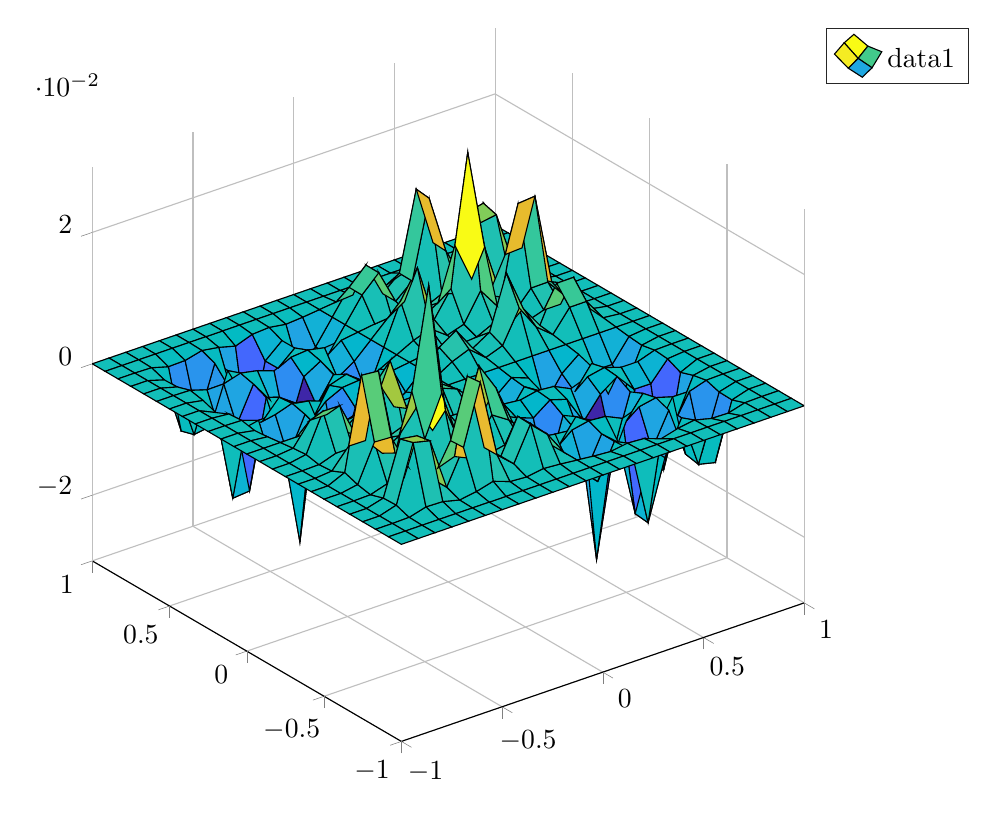
\begin{tikzpicture}

\begin{axis}[%
width=3.56in,
height=3.566in,
at={(0.597in,0.481in)},
scale only axis,
xmin=-1,
xmax=1,
tick align=outside,
ymin=-1,
ymax=1,
zmin=-0.03,
zmax=0.03,
view={-37.5}{30},
axis background/.style={fill=white},
axis x line*=bottom,
axis y line*=left,
axis z line*=left,
xmajorgrids,
ymajorgrids,
zmajorgrids,
legend style={at={(1.03,1)}, anchor=north west, legend cell align=left, align=left, draw=white!15!black}
]

\addplot3[%
surf,
shader=flat corner, draw=black, z buffer=sort, colormap={mymap}{[1pt] rgb(0pt)=(0.2422,0.1504,0.6603); rgb(1pt)=(0.25039,0.164995,0.707614); rgb(2pt)=(0.257771,0.181781,0.751138); rgb(3pt)=(0.264729,0.197757,0.795214); rgb(4pt)=(0.270648,0.214676,0.836371); rgb(5pt)=(0.275114,0.234238,0.870986); rgb(6pt)=(0.2783,0.255871,0.899071); rgb(7pt)=(0.280333,0.278233,0.9221); rgb(8pt)=(0.281338,0.300595,0.941376); rgb(9pt)=(0.281014,0.322757,0.957886); rgb(10pt)=(0.279467,0.344671,0.971676); rgb(11pt)=(0.275971,0.366681,0.982905); rgb(12pt)=(0.269914,0.3892,0.9906); rgb(13pt)=(0.260243,0.412329,0.995157); rgb(14pt)=(0.244033,0.435833,0.998833); rgb(15pt)=(0.220643,0.460257,0.997286); rgb(16pt)=(0.196333,0.484719,0.989152); rgb(17pt)=(0.183405,0.507371,0.979795); rgb(18pt)=(0.178643,0.528857,0.968157); rgb(19pt)=(0.176438,0.549905,0.952019); rgb(20pt)=(0.168743,0.570262,0.935871); rgb(21pt)=(0.154,0.5902,0.9218); rgb(22pt)=(0.146029,0.609119,0.907857); rgb(23pt)=(0.138024,0.627629,0.89729); rgb(24pt)=(0.124814,0.645929,0.888343); rgb(25pt)=(0.111252,0.6635,0.876314); rgb(26pt)=(0.0952095,0.679829,0.859781); rgb(27pt)=(0.0688714,0.694771,0.839357); rgb(28pt)=(0.0296667,0.708167,0.816333); rgb(29pt)=(0.00357143,0.720267,0.7917); rgb(30pt)=(0.00665714,0.731214,0.766014); rgb(31pt)=(0.0433286,0.741095,0.73941); rgb(32pt)=(0.0963952,0.75,0.712038); rgb(33pt)=(0.140771,0.7584,0.684157); rgb(34pt)=(0.1717,0.766962,0.655443); rgb(35pt)=(0.193767,0.775767,0.6251); rgb(36pt)=(0.216086,0.7843,0.5923); rgb(37pt)=(0.246957,0.791795,0.556743); rgb(38pt)=(0.290614,0.79729,0.518829); rgb(39pt)=(0.340643,0.8008,0.478857); rgb(40pt)=(0.3909,0.802871,0.435448); rgb(41pt)=(0.445629,0.802419,0.390919); rgb(42pt)=(0.5044,0.7993,0.348); rgb(43pt)=(0.561562,0.794233,0.304481); rgb(44pt)=(0.617395,0.787619,0.261238); rgb(45pt)=(0.671986,0.779271,0.2227); rgb(46pt)=(0.7242,0.769843,0.191029); rgb(47pt)=(0.773833,0.759805,0.16461); rgb(48pt)=(0.820314,0.749814,0.153529); rgb(49pt)=(0.863433,0.7406,0.159633); rgb(50pt)=(0.903543,0.733029,0.177414); rgb(51pt)=(0.939257,0.728786,0.209957); rgb(52pt)=(0.972757,0.729771,0.239443); rgb(53pt)=(0.995648,0.743371,0.237148); rgb(54pt)=(0.996986,0.765857,0.219943); rgb(55pt)=(0.995205,0.789252,0.202762); rgb(56pt)=(0.9892,0.813567,0.188533); rgb(57pt)=(0.978629,0.838629,0.176557); rgb(58pt)=(0.967648,0.8639,0.16429); rgb(59pt)=(0.96101,0.889019,0.153676); rgb(60pt)=(0.959671,0.913457,0.142257); rgb(61pt)=(0.962795,0.937338,0.12651); rgb(62pt)=(0.969114,0.960629,0.106362); rgb(63pt)=(0.9769,0.9839,0.0805)}, mesh/rows=25]
table[row sep=crcr, point meta=\thisrow{c}] {%
%
x	y	z	c\\
-1	-1	0	0\\
-0.916666666666667	-1	0	0\\
-0.833333333333333	-1	1.02695723625141e-24	1.02695723625141e-24\\
-0.75	-1	0	0\\
-0.666666666666667	-1	0	0\\
-0.583333333333333	-1	0	0\\
-0.5	-1	0	0\\
-0.416666666666667	-1	0	0\\
-0.333333333333333	-1	0	0\\
-0.25	-1	0	0\\
-0.166666666666667	-1	0	0\\
-0.0833333333333334	-1	0	0\\
0	-1	0	0\\
0.0833333333333333	-1	0	0\\
0.166666666666667	-1	0	0\\
0.25	-1	0	0\\
0.333333333333333	-1	0	0\\
0.416666666666667	-1	0	0\\
0.5	-1	0	0\\
0.583333333333333	-1	0	0\\
0.666666666666667	-1	0	0\\
0.75	-1	0	0\\
0.833333333333333	-1	0	0\\
0.916666666666667	-1	-4.38399307163469e-27	-4.38399307163469e-27\\
1	-1	0	0\\
-1	-0.916666666666667	0	0\\
-0.916666666666667	-0.916666666666667	2.55753406345044e-09	2.55753406345044e-09\\
-0.833333333333333	-0.916666666666667	3.85777718973534e-07	3.85777718973534e-07\\
-0.75	-0.916666666666667	4.17100875631788e-06	4.17100875631788e-06\\
-0.666666666666667	-0.916666666666667	3.64929550800072e-06	3.64929550800072e-06\\
-0.583333333333333	-0.916666666666667	3.45860111752149e-07	3.45860111752149e-07\\
-0.5	-0.916666666666667	2.33954300020683e-06	2.33954300020683e-06\\
-0.416666666666667	-0.916666666666667	5.70854139583692e-06	5.70854139583692e-06\\
-0.333333333333333	-0.916666666666667	1.17920908563584e-06	1.17920908563584e-06\\
-0.25	-0.916666666666667	3.45029265806706e-07	3.45029265806706e-07\\
-0.166666666666667	-0.916666666666667	2.26755661545572e-06	2.26755661545572e-06\\
-0.0833333333333334	-0.916666666666667	1.33785564740444e-06	1.33785564740444e-06\\
0	-0.916666666666667	-4.2425755489483e-22	-4.2425755489483e-22\\
0.0833333333333333	-0.916666666666667	-1.33785564740444e-06	-1.33785564740444e-06\\
0.166666666666667	-0.916666666666667	-2.26755661545571e-06	-2.26755661545571e-06\\
0.25	-0.916666666666667	-3.45029265806705e-07	-3.45029265806705e-07\\
0.333333333333333	-0.916666666666667	-1.17920908563584e-06	-1.17920908563584e-06\\
0.416666666666667	-0.916666666666667	-5.70854139583693e-06	-5.70854139583693e-06\\
0.5	-0.916666666666667	-2.33954300020683e-06	-2.33954300020683e-06\\
0.583333333333333	-0.916666666666667	-3.4586011175215e-07	-3.4586011175215e-07\\
0.666666666666667	-0.916666666666667	-3.64929550800072e-06	-3.64929550800072e-06\\
0.75	-0.916666666666667	-4.17100875631788e-06	-4.17100875631788e-06\\
0.833333333333333	-0.916666666666667	-3.85777718973533e-07	-3.85777718973533e-07\\
0.916666666666667	-0.916666666666667	-2.55753406345042e-09	-2.55753406345042e-09\\
1	-0.916666666666667	0	0\\
-1	-0.833333333333333	1.02695723625141e-24	1.02695723625141e-24\\
-0.916666666666667	-0.833333333333333	3.85777718973533e-07	3.85777718973533e-07\\
-0.833333333333333	-0.833333333333333	6.71198962422951e-05	6.71198962422951e-05\\
-0.75	-0.833333333333333	0.000778127800887982	0.000778127800887982\\
-0.666666666666667	-0.833333333333333	0.000707315736756557	0.000707315736756557\\
-0.583333333333333	-0.833333333333333	6.86074746915453e-05	6.86074746915453e-05\\
-0.5	-0.833333333333333	0.000471138162446881	0.000471138162446881\\
-0.416666666666667	-0.833333333333333	0.00116140316014542	0.00116140316014542\\
-0.333333333333333	-0.833333333333333	0.000241610914204461	0.000241610914204461\\
-0.25	-0.833333333333333	7.10368896279139e-05	7.10368896279139e-05\\
-0.166666666666667	-0.833333333333333	0.000468336406285743	0.000468336406285743\\
-0.0833333333333334	-0.833333333333333	0.000276812375771035	0.000276812375771035\\
0	-0.833333333333333	-7.74552301490904e-20	-7.74552301490904e-20\\
0.0833333333333333	-0.833333333333333	-0.000276812375771035	-0.000276812375771035\\
0.166666666666667	-0.833333333333333	-0.000468336406285742	-0.000468336406285742\\
0.25	-0.833333333333333	-7.10368896279136e-05	-7.10368896279136e-05\\
0.333333333333333	-0.833333333333333	-0.00024161091420446	-0.00024161091420446\\
0.416666666666667	-0.833333333333333	-0.00116140316014542	-0.00116140316014542\\
0.5	-0.833333333333333	-0.000471138162446881	-0.000471138162446881\\
0.583333333333333	-0.833333333333333	-6.86074746915456e-05	-6.86074746915456e-05\\
0.666666666666667	-0.833333333333333	-0.000707315736756559	-0.000707315736756559\\
0.75	-0.833333333333333	-0.000778127800887981	-0.000778127800887981\\
0.833333333333333	-0.833333333333333	-6.7119896242295e-05	-6.7119896242295e-05\\
0.916666666666667	-0.833333333333333	-3.85777718973525e-07	-3.85777718973525e-07\\
1	-0.833333333333333	-1.0269572362514e-24	-1.0269572362514e-24\\
-1	-0.75	0	0\\
-0.916666666666667	-0.75	4.17100875631788e-06	4.17100875631788e-06\\
-0.833333333333333	-0.75	0.000778127800887983	0.000778127800887983\\
-0.75	-0.75	0.00943571698715445	0.00943571698715445\\
-0.666666666666667	-0.75	0.00882480124123988	0.00882480124123988\\
-0.583333333333333	-0.75	0.000872104526134152	0.000872104526134152\\
-0.5	-0.75	0.0060652983794619	0.0060652983794619\\
-0.416666666666667	-0.75	0.0150841772008774	0.0150841772008774\\
-0.333333333333333	-0.75	0.00315753528677166	0.00315753528677166\\
-0.25	-0.75	0.000932352964394895	0.000932352964394895\\
-0.166666666666667	-0.75	0.00616423466770155	0.00616423466770155\\
-0.0833333333333334	-0.75	0.00364924259814257	0.00364924259814257\\
0	-0.75	-8.76737641779841e-19	-8.76737641779841e-19\\
0.0833333333333333	-0.75	-0.00364924259814257	-0.00364924259814257\\
0.166666666666667	-0.75	-0.00616423466770154	-0.00616423466770154\\
0.25	-0.75	-0.000932352964394891	-0.000932352964394891\\
0.333333333333333	-0.75	-0.00315753528677164	-0.00315753528677164\\
0.416666666666667	-0.75	-0.0150841772008774	-0.0150841772008774\\
0.5	-0.75	-0.0060652983794619	-0.0060652983794619\\
0.583333333333333	-0.75	-0.000872104526134156	-0.000872104526134156\\
0.666666666666667	-0.75	-0.00882480124123989	-0.00882480124123989\\
0.75	-0.75	-0.00943571698715444	-0.00943571698715444\\
0.833333333333333	-0.75	-0.000778127800887982	-0.000778127800887982\\
0.916666666666667	-0.75	-4.17100875631781e-06	-4.17100875631781e-06\\
1	-0.75	0	0\\
-1	-0.666666666666667	0	0\\
-0.916666666666667	-0.666666666666667	3.64929550800072e-06	3.64929550800072e-06\\
-0.833333333333333	-0.666666666666667	0.000707315736756557	0.000707315736756557\\
-0.75	-0.666666666666667	0.00882480124123988	0.00882480124123988\\
-0.666666666666667	-0.666666666666667	0.00842066215543398	0.00842066215543398\\
-0.583333333333333	-0.666666666666667	0.000843966898384536	0.000843966898384536\\
-0.5	-0.666666666666667	0.00592857826938018	0.00592857826938018\\
-0.416666666666667	-0.666666666666667	0.0148502404760497	0.0148502404760497\\
-0.333333333333333	-0.666666666666667	0.00312456184123599	0.00312456184123599\\
-0.25	-0.666666666666667	0.000925942478032866	0.000925942478032866\\
-0.166666666666667	-0.666666666666667	0.00613646636398126	0.00613646636398126\\
-0.0833333333333334	-0.666666666666667	0.00363775449063844	0.00363775449063844\\
0	-0.666666666666667	-8.44331861748012e-19	-8.44331861748012e-19\\
0.0833333333333333	-0.666666666666667	-0.00363775449063844	-0.00363775449063844\\
0.166666666666667	-0.666666666666667	-0.00613646636398124	-0.00613646636398124\\
0.25	-0.666666666666667	-0.000925942478032862	-0.000925942478032862\\
0.333333333333333	-0.666666666666667	-0.00312456184123597	-0.00312456184123597\\
0.416666666666667	-0.666666666666667	-0.0148502404760497	-0.0148502404760497\\
0.5	-0.666666666666667	-0.00592857826938018	-0.00592857826938018\\
0.583333333333333	-0.666666666666667	-0.00084396689838454	-0.00084396689838454\\
0.666666666666667	-0.666666666666667	-0.00842066215543399	-0.00842066215543399\\
0.75	-0.666666666666667	-0.00882480124123987	-0.00882480124123987\\
0.833333333333333	-0.666666666666667	-0.000707315736756558	-0.000707315736756558\\
0.916666666666667	-0.666666666666667	-3.64929550800066e-06	-3.64929550800066e-06\\
1	-0.666666666666667	0	0\\
-1	-0.583333333333333	0	0\\
-0.916666666666667	-0.583333333333333	3.45860111752149e-07	3.45860111752149e-07\\
-0.833333333333333	-0.583333333333333	6.86074746915453e-05	6.86074746915453e-05\\
-0.75	-0.583333333333333	0.000872104526134152	0.000872104526134152\\
-0.666666666666667	-0.583333333333333	0.000843966898384536	0.000843966898384536\\
-0.583333333333333	-0.583333333333333	8.50681297213606e-05	8.50681297213606e-05\\
-0.5	-0.583333333333333	0.000592761470027727	0.000592761470027727\\
-0.416666666666667	-0.583333333333333	0.00149315597727987	0.00149315597727987\\
-0.333333333333333	-0.583333333333333	0.000315453871556334	0.000315453871556334\\
-0.25	-0.583333333333333	9.31814902686496e-05	9.31814902686496e-05\\
-0.166666666666667	-0.583333333333333	0.000618502248354859	0.000618502248354859\\
-0.0833333333333334	-0.583333333333333	0.000367064223668659	0.000367064223668659\\
0	-0.583333333333333	-7.40930762219607e-20	-7.40930762219607e-20\\
0.0833333333333333	-0.583333333333333	-0.000367064223668659	-0.000367064223668659\\
0.166666666666667	-0.583333333333333	-0.000618502248354857	-0.000618502248354857\\
0.25	-0.583333333333333	-9.31814902686491e-05	-9.31814902686491e-05\\
0.333333333333333	-0.583333333333333	-0.000315453871556332	-0.000315453871556332\\
0.416666666666667	-0.583333333333333	-0.00149315597727987	-0.00149315597727987\\
0.5	-0.583333333333333	-0.000592761470027727	-0.000592761470027727\\
0.583333333333333	-0.583333333333333	-8.50681297213611e-05	-8.50681297213611e-05\\
0.666666666666667	-0.583333333333333	-0.000843966898384538	-0.000843966898384538\\
0.75	-0.583333333333333	-0.00087210452613415	-0.00087210452613415\\
0.833333333333333	-0.583333333333333	-6.86074746915454e-05	-6.86074746915454e-05\\
0.916666666666667	-0.583333333333333	-3.45860111752143e-07	-3.45860111752143e-07\\
1	-0.583333333333333	0	0\\
-1	-0.5	0	0\\
-0.916666666666667	-0.5	2.33954300020683e-06	2.33954300020683e-06\\
-0.833333333333333	-0.5	0.000471138162446881	0.000471138162446881\\
-0.75	-0.5	0.0060652983794619	0.0060652983794619\\
-0.666666666666667	-0.5	0.00592857826938018	0.00592857826938018\\
-0.583333333333333	-0.5	0.000592761470027727	0.000592761470027727\\
-0.5	-0.5	0.00393294666281547	0.00393294666281547\\
-0.416666666666667	-0.5	0.00994977833558941	0.00994977833558941\\
-0.333333333333333	-0.5	0.00210867680461956	0.00210867680461956\\
-0.25	-0.5	0.000610455051438689	0.000610455051438689\\
-0.166666666666667	-0.5	0.00405241439845992	0.00405241439845992\\
-0.0833333333333334	-0.5	0.0024071556172955	0.0024071556172955\\
0	-0.5	-5.91805759022251e-19	-5.91805759022251e-19\\
0.0833333333333333	-0.5	-0.0024071556172955	-0.0024071556172955\\
0.166666666666667	-0.5	-0.00405241439845991	-0.00405241439845991\\
0.25	-0.5	-0.000610455051438686	-0.000610455051438686\\
0.333333333333333	-0.5	-0.00210867680461956	-0.00210867680461956\\
0.416666666666667	-0.5	-0.00994977833558942	-0.00994977833558942\\
0.5	-0.5	-0.00393294666281547	-0.00393294666281547\\
0.583333333333333	-0.5	-0.000592761470027729	-0.000592761470027729\\
0.666666666666667	-0.5	-0.00592857826938019	-0.00592857826938019\\
0.75	-0.5	-0.00606529837946189	-0.00606529837946189\\
0.833333333333333	-0.5	-0.000471138162446881	-0.000471138162446881\\
0.916666666666667	-0.5	-2.33954300020679e-06	-2.33954300020679e-06\\
1	-0.5	0	0\\
-1	-0.416666666666667	0	0\\
-0.916666666666667	-0.416666666666667	5.70854139583692e-06	5.70854139583692e-06\\
-0.833333333333333	-0.416666666666667	0.00116140316014542	0.00116140316014542\\
-0.75	-0.416666666666667	0.0150841772008774	0.0150841772008774\\
-0.666666666666667	-0.416666666666667	0.0148502404760497	0.0148502404760497\\
-0.583333333333333	-0.416666666666667	0.00149315597727987	0.00149315597727987\\
-0.5	-0.416666666666667	0.00994977833558941	0.00994977833558941\\
-0.416666666666667	-0.416666666666667	0.0252552578198303	0.0252552578198303\\
-0.333333333333333	-0.416666666666667	0.00536572588063085	0.00536572588063085\\
-0.25	-0.416666666666667	0.00155612453270233	0.00155612453270233\\
-0.166666666666667	-0.416666666666667	0.010342674976464	0.010342674976464\\
-0.0833333333333334	-0.416666666666667	0.00614793627719881	0.00614793627719881\\
0	-0.416666666666667	-1.50433859765667e-18	-1.50433859765667e-18\\
0.0833333333333333	-0.416666666666667	-0.0061479362771988	-0.0061479362771988\\
0.166666666666667	-0.416666666666667	-0.010342674976464	-0.010342674976464\\
0.25	-0.416666666666667	-0.00155612453270232	-0.00155612453270232\\
0.333333333333333	-0.416666666666667	-0.00536572588063083	-0.00536572588063083\\
0.416666666666667	-0.416666666666667	-0.0252552578198304	-0.0252552578198304\\
0.5	-0.416666666666667	-0.00994977833558941	-0.00994977833558941\\
0.583333333333333	-0.416666666666667	-0.00149315597727988	-0.00149315597727988\\
0.666666666666667	-0.416666666666667	-0.0148502404760497	-0.0148502404760497\\
0.75	-0.416666666666667	-0.0150841772008774	-0.0150841772008774\\
0.833333333333333	-0.416666666666667	-0.00116140316014542	-0.00116140316014542\\
0.916666666666667	-0.416666666666667	-5.70854139583682e-06	-5.70854139583682e-06\\
1	-0.416666666666667	0	0\\
-1	-0.333333333333333	0	0\\
-0.916666666666667	-0.333333333333333	1.17920908563584e-06	1.17920908563584e-06\\
-0.833333333333333	-0.333333333333333	0.000241610914204461	0.000241610914204461\\
-0.75	-0.333333333333333	0.00315753528677166	0.00315753528677166\\
-0.666666666666667	-0.333333333333333	0.00312456184123599	0.00312456184123599\\
-0.583333333333333	-0.333333333333333	0.000315453871556334	0.000315453871556334\\
-0.5	-0.333333333333333	0.00210867680461956	0.00210867680461956\\
-0.416666666666667	-0.333333333333333	0.00536572588063085	0.00536572588063085\\
-0.333333333333333	-0.333333333333333	0.00114214387023767	0.00114214387023767\\
-0.25	-0.333333333333333	0.000331677317790113	0.000331677317790113\\
-0.166666666666667	-0.333333333333333	0.00220651736235955	0.00220651736235955\\
-0.0833333333333334	-0.333333333333333	0.00131231582712499	0.00131231582712499\\
0	-0.333333333333333	-3.16585135024486e-19	-3.16585135024486e-19\\
0.0833333333333333	-0.333333333333333	-0.00131231582712499	-0.00131231582712499\\
0.166666666666667	-0.333333333333333	-0.00220651736235954	-0.00220651736235954\\
0.25	-0.333333333333333	-0.000331677317790112	-0.000331677317790112\\
0.333333333333333	-0.333333333333333	-0.00114214387023766	-0.00114214387023766\\
0.416666666666667	-0.333333333333333	-0.00536572588063086	-0.00536572588063086\\
0.5	-0.333333333333333	-0.00210867680461956	-0.00210867680461956\\
0.583333333333333	-0.333333333333333	-0.000315453871556335	-0.000315453871556335\\
0.666666666666667	-0.333333333333333	-0.00312456184123599	-0.00312456184123599\\
0.75	-0.333333333333333	-0.00315753528677165	-0.00315753528677165\\
0.833333333333333	-0.333333333333333	-0.000241610914204461	-0.000241610914204461\\
0.916666666666667	-0.333333333333333	-1.17920908563582e-06	-1.17920908563582e-06\\
1	-0.333333333333333	0	0\\
-1	-0.25	0	0\\
-0.916666666666667	-0.25	3.45029265806706e-07	3.45029265806706e-07\\
-0.833333333333333	-0.25	7.1036889627914e-05	7.1036889627914e-05\\
-0.75	-0.25	0.000932352964394894	0.000932352964394894\\
-0.666666666666667	-0.25	0.000925942478032866	0.000925942478032866\\
-0.583333333333333	-0.25	9.31814902686495e-05	9.31814902686495e-05\\
-0.5	-0.25	0.000610455051438689	0.000610455051438689\\
-0.416666666666667	-0.25	0.00155612453270233	0.00155612453270233\\
-0.333333333333333	-0.25	0.000331677317790113	0.000331677317790113\\
-0.25	-0.25	9.54350634367825e-05	9.54350634367825e-05\\
-0.166666666666667	-0.25	0.000634901021554919	0.000634901021554919\\
-0.0833333333333334	-0.25	0.00037775454883306	0.00037775454883306\\
0	-0.25	-8.80499813311504e-20	-8.80499813311504e-20\\
0.0833333333333333	-0.25	-0.00037775454883306	-0.00037775454883306\\
0.166666666666667	-0.25	-0.000634901021554917	-0.000634901021554917\\
0.25	-0.25	-9.54350634367821e-05	-9.54350634367821e-05\\
0.333333333333333	-0.25	-0.000331677317790112	-0.000331677317790112\\
0.416666666666667	-0.25	-0.00155612453270233	-0.00155612453270233\\
0.5	-0.25	-0.000610455051438689	-0.000610455051438689\\
0.583333333333333	-0.25	-9.31814902686498e-05	-9.31814902686498e-05\\
0.666666666666667	-0.25	-0.000925942478032867	-0.000925942478032867\\
0.75	-0.25	-0.000932352964394893	-0.000932352964394893\\
0.833333333333333	-0.25	-7.1036889627914e-05	-7.1036889627914e-05\\
0.916666666666667	-0.25	-3.450292658067e-07	-3.450292658067e-07\\
1	-0.25	0	0\\
-1	-0.166666666666667	0	0\\
-0.916666666666667	-0.166666666666667	2.26755661545572e-06	2.26755661545572e-06\\
-0.833333333333333	-0.166666666666667	0.000468336406285743	0.000468336406285743\\
-0.75	-0.166666666666667	0.00616423466770155	0.00616423466770155\\
-0.666666666666667	-0.166666666666667	0.00613646636398126	0.00613646636398126\\
-0.583333333333333	-0.166666666666667	0.000618502248354858	0.000618502248354858\\
-0.5	-0.166666666666667	0.00405241439845992	0.00405241439845992\\
-0.416666666666667	-0.166666666666667	0.010342674976464	0.010342674976464\\
-0.333333333333333	-0.166666666666667	0.00220651736235955	0.00220651736235955\\
-0.25	-0.166666666666667	0.000634901021554919	0.000634901021554919\\
-0.166666666666667	-0.166666666666667	0.00422559650685534	0.00422559650685534\\
-0.0833333333333334	-0.166666666666667	0.00251483803933617	0.00251483803933617\\
0	-0.166666666666667	-6.34758211468699e-19	-6.34758211468699e-19\\
0.0833333333333333	-0.166666666666667	-0.00251483803933617	-0.00251483803933617\\
0.166666666666667	-0.166666666666667	-0.00422559650685533	-0.00422559650685533\\
0.25	-0.166666666666667	-0.000634901021554916	-0.000634901021554916\\
0.333333333333333	-0.166666666666667	-0.00220651736235954	-0.00220651736235954\\
0.416666666666667	-0.166666666666667	-0.010342674976464	-0.010342674976464\\
0.5	-0.166666666666667	-0.00405241439845992	-0.00405241439845992\\
0.583333333333333	-0.166666666666667	-0.000618502248354861	-0.000618502248354861\\
0.666666666666667	-0.166666666666667	-0.00613646636398127	-0.00613646636398127\\
0.75	-0.166666666666667	-0.00616423466770154	-0.00616423466770154\\
0.833333333333333	-0.166666666666667	-0.000468336406285743	-0.000468336406285743\\
0.916666666666667	-0.166666666666667	-2.26755661545568e-06	-2.26755661545568e-06\\
1	-0.166666666666667	0	0\\
-1	-0.0833333333333334	0	0\\
-0.916666666666667	-0.0833333333333334	1.33785564740444e-06	1.33785564740444e-06\\
-0.833333333333333	-0.0833333333333334	0.000276812375771035	0.000276812375771035\\
-0.75	-0.0833333333333334	0.00364924259814257	0.00364924259814257\\
-0.666666666666667	-0.0833333333333334	0.00363775449063844	0.00363775449063844\\
-0.583333333333333	-0.0833333333333334	0.000367064223668659	0.000367064223668659\\
-0.5	-0.0833333333333334	0.0024071556172955	0.0024071556172955\\
-0.416666666666667	-0.0833333333333334	0.0061479362771988	0.0061479362771988\\
-0.333333333333333	-0.0833333333333334	0.00131231582712499	0.00131231582712499\\
-0.25	-0.0833333333333334	0.00037775454883306	0.00037775454883306\\
-0.166666666666667	-0.0833333333333334	0.00251483803933617	0.00251483803933617\\
-0.0833333333333334	-0.0833333333333334	0.0014969284339611	0.0014969284339611\\
0	-0.0833333333333334	-4.12134423225633e-19	-4.12134423225633e-19\\
0.0833333333333333	-0.0833333333333334	-0.0014969284339611	-0.0014969284339611\\
0.166666666666667	-0.0833333333333334	-0.00251483803933616	-0.00251483803933616\\
0.25	-0.0833333333333334	-0.000377754548833058	-0.000377754548833058\\
0.333333333333333	-0.0833333333333334	-0.00131231582712498	-0.00131231582712498\\
0.416666666666667	-0.0833333333333334	-0.00614793627719881	-0.00614793627719881\\
0.5	-0.0833333333333334	-0.00240715561729551	-0.00240715561729551\\
0.583333333333333	-0.0833333333333334	-0.000367064223668661	-0.000367064223668661\\
0.666666666666667	-0.0833333333333334	-0.00363775449063844	-0.00363775449063844\\
0.75	-0.0833333333333334	-0.00364924259814256	-0.00364924259814256\\
0.833333333333333	-0.0833333333333334	-0.000276812375771035	-0.000276812375771035\\
0.916666666666667	-0.0833333333333334	-1.33785564740442e-06	-1.33785564740442e-06\\
1	-0.0833333333333334	0	0\\
-1	0	0	0\\
-0.916666666666667	0	-4.22019650749432e-22	-4.22019650749432e-22\\
-0.833333333333333	0	-7.58062703141482e-20	-7.58062703141482e-20\\
-0.75	0	-8.8948973557021e-19	-8.8948973557021e-19\\
-0.666666666666667	0	-8.48925864908015e-19	-8.48925864908015e-19\\
-0.583333333333333	0	-7.4663668535476e-20	-7.4663668535476e-20\\
-0.5	0	-6.59299545930563e-19	-6.59299545930563e-19\\
-0.416666666666667	0	-1.65655633099897e-18	-1.65655633099897e-18\\
-0.333333333333333	0	-3.57084812293917e-19	-3.57084812293917e-19\\
-0.25	0	-8.37743870326049e-20	-8.37743870326049e-20\\
-0.166666666666667	0	-6.03879200828298e-19	-6.03879200828298e-19\\
-0.0833333333333334	0	-3.932851103973e-19	-3.932851103973e-19\\
0	0	-4.82118586296267e-21	-4.82118586296267e-21\\
0.0833333333333333	0	4.48056541275829e-19	4.48056541275829e-19\\
0.166666666666667	0	6.75165917404855e-19	6.75165917404855e-19\\
0.25	0	8.05379513898792e-20	8.05379513898792e-20\\
0.333333333333333	0	3.00487456194101e-19	3.00487456194101e-19\\
0.416666666666667	0	1.62580333661468e-18	1.62580333661468e-18\\
0.5	0	5.57212921187685e-19	5.57212921187685e-19\\
0.583333333333333	0	9.80093456331336e-20	9.80093456331336e-20\\
0.666666666666667	0	8.61737011716055e-19	8.61737011716055e-19\\
0.75	0	9.60761298722394e-19	9.60761298722394e-19\\
0.833333333333333	0	7.99192795843061e-20	7.99192795843061e-20\\
0.916666666666667	0	3.15236993062634e-22	3.15236993062634e-22\\
1	0	0	0\\
-1	0.0833333333333333	0	0\\
-0.916666666666667	0.0833333333333333	-1.33785564740444e-06	-1.33785564740444e-06\\
-0.833333333333333	0.0833333333333333	-0.000276812375771035	-0.000276812375771035\\
-0.75	0.0833333333333333	-0.00364924259814257	-0.00364924259814257\\
-0.666666666666667	0.0833333333333333	-0.00363775449063844	-0.00363775449063844\\
-0.583333333333333	0.0833333333333333	-0.000367064223668659	-0.000367064223668659\\
-0.5	0.0833333333333333	-0.0024071556172955	-0.0024071556172955\\
-0.416666666666667	0.0833333333333333	-0.0061479362771988	-0.0061479362771988\\
-0.333333333333333	0.0833333333333333	-0.00131231582712499	-0.00131231582712499\\
-0.25	0.0833333333333333	-0.00037775454883306	-0.00037775454883306\\
-0.166666666666667	0.0833333333333333	-0.00251483803933617	-0.00251483803933617\\
-0.0833333333333334	0.0833333333333333	-0.0014969284339611	-0.0014969284339611\\
0	0.0833333333333333	4.51410925247731e-19	4.51410925247731e-19\\
0.0833333333333333	0.0833333333333333	0.0014969284339611	0.0014969284339611\\
0.166666666666667	0.0833333333333333	0.00251483803933616	0.00251483803933616\\
0.25	0.0833333333333333	0.000377754548833058	0.000377754548833058\\
0.333333333333333	0.0833333333333333	0.00131231582712498	0.00131231582712498\\
0.416666666666667	0.0833333333333333	0.00614793627719881	0.00614793627719881\\
0.5	0.0833333333333333	0.0024071556172955	0.0024071556172955\\
0.583333333333333	0.0833333333333333	0.00036706422366866	0.00036706422366866\\
0.666666666666667	0.0833333333333333	0.00363775449063844	0.00363775449063844\\
0.75	0.0833333333333333	0.00364924259814256	0.00364924259814256\\
0.833333333333333	0.0833333333333333	0.000276812375771035	0.000276812375771035\\
0.916666666666667	0.0833333333333333	1.33785564740442e-06	1.33785564740442e-06\\
1	0.0833333333333333	0	0\\
-1	0.166666666666667	0	0\\
-0.916666666666667	0.166666666666667	-2.26755661545571e-06	-2.26755661545571e-06\\
-0.833333333333333	0.166666666666667	-0.000468336406285741	-0.000468336406285741\\
-0.75	0.166666666666667	-0.00616423466770153	-0.00616423466770153\\
-0.666666666666667	0.166666666666667	-0.00613646636398124	-0.00613646636398124\\
-0.583333333333333	0.166666666666667	-0.000618502248354857	-0.000618502248354857\\
-0.5	0.166666666666667	-0.00405241439845991	-0.00405241439845991\\
-0.416666666666667	0.166666666666667	-0.010342674976464	-0.010342674976464\\
-0.333333333333333	0.166666666666667	-0.00220651736235954	-0.00220651736235954\\
-0.25	0.166666666666667	-0.000634901021554917	-0.000634901021554917\\
-0.166666666666667	0.166666666666667	-0.00422559650685533	-0.00422559650685533\\
-0.0833333333333334	0.166666666666667	-0.00251483803933616	-0.00251483803933616\\
0	0.166666666666667	6.9848421185914e-19	6.9848421185914e-19\\
0.0833333333333333	0.166666666666667	0.00251483803933616	0.00251483803933616\\
0.166666666666667	0.166666666666667	0.00422559650685532	0.00422559650685532\\
0.25	0.166666666666667	0.000634901021554914	0.000634901021554914\\
0.333333333333333	0.166666666666667	0.00220651736235953	0.00220651736235953\\
0.416666666666667	0.166666666666667	0.010342674976464	0.010342674976464\\
0.5	0.166666666666667	0.00405241439845991	0.00405241439845991\\
0.583333333333333	0.166666666666667	0.000618502248354859	0.000618502248354859\\
0.666666666666667	0.166666666666667	0.00613646636398125	0.00613646636398125\\
0.75	0.166666666666667	0.00616423466770152	0.00616423466770152\\
0.833333333333333	0.166666666666667	0.000468336406285741	0.000468336406285741\\
0.916666666666667	0.166666666666667	2.26755661545567e-06	2.26755661545567e-06\\
1	0.166666666666667	0	0\\
-1	0.25	0	0\\
-0.916666666666667	0.25	-3.45029265806704e-07	-3.45029265806704e-07\\
-0.833333333333333	0.25	-7.10368896279136e-05	-7.10368896279136e-05\\
-0.75	0.25	-0.000932352964394891	-0.000932352964394891\\
-0.666666666666667	0.25	-0.000925942478032862	-0.000925942478032862\\
-0.583333333333333	0.25	-9.31814902686491e-05	-9.31814902686491e-05\\
-0.5	0.25	-0.000610455051438686	-0.000610455051438686\\
-0.416666666666667	0.25	-0.00155612453270232	-0.00155612453270232\\
-0.333333333333333	0.25	-0.000331677317790112	-0.000331677317790112\\
-0.25	0.25	-9.5435063436782e-05	-9.5435063436782e-05\\
-0.166666666666667	0.25	-0.000634901021554916	-0.000634901021554916\\
-0.0833333333333334	0.25	-0.000377754548833058	-0.000377754548833058\\
0	0.25	7.94089675468141e-20	7.94089675468141e-20\\
0.0833333333333333	0.25	0.000377754548833058	0.000377754548833058\\
0.166666666666667	0.25	0.000634901021554914	0.000634901021554914\\
0.25	0.25	9.54350634367817e-05	9.54350634367817e-05\\
0.333333333333333	0.25	0.000331677317790111	0.000331677317790111\\
0.416666666666667	0.25	0.00155612453270232	0.00155612453270232\\
0.5	0.25	0.000610455051438686	0.000610455051438686\\
0.583333333333333	0.25	9.31814902686495e-05	9.31814902686495e-05\\
0.666666666666667	0.25	0.000925942478032864	0.000925942478032864\\
0.75	0.25	0.000932352964394889	0.000932352964394889\\
0.833333333333333	0.25	7.10368896279137e-05	7.10368896279137e-05\\
0.916666666666667	0.25	3.45029265806699e-07	3.45029265806699e-07\\
1	0.25	0	0\\
-1	0.333333333333333	0	0\\
-0.916666666666667	0.333333333333333	-1.17920908563583e-06	-1.17920908563583e-06\\
-0.833333333333333	0.333333333333333	-0.00024161091420446	-0.00024161091420446\\
-0.75	0.333333333333333	-0.00315753528677164	-0.00315753528677164\\
-0.666666666666667	0.333333333333333	-0.00312456184123597	-0.00312456184123597\\
-0.583333333333333	0.333333333333333	-0.000315453871556332	-0.000315453871556332\\
-0.5	0.333333333333333	-0.00210867680461956	-0.00210867680461956\\
-0.416666666666667	0.333333333333333	-0.00536572588063083	-0.00536572588063083\\
-0.333333333333333	0.333333333333333	-0.00114214387023766	-0.00114214387023766\\
-0.25	0.333333333333333	-0.000331677317790112	-0.000331677317790112\\
-0.166666666666667	0.333333333333333	-0.00220651736235954	-0.00220651736235954\\
-0.0833333333333334	0.333333333333333	-0.00131231582712498	-0.00131231582712498\\
0	0.333333333333333	3.22485562489602e-19	3.22485562489602e-19\\
0.0833333333333333	0.333333333333333	0.00131231582712498	0.00131231582712498\\
0.166666666666667	0.333333333333333	0.00220651736235953	0.00220651736235953\\
0.25	0.333333333333333	0.000331677317790111	0.000331677317790111\\
0.333333333333333	0.333333333333333	0.00114214387023766	0.00114214387023766\\
0.416666666666667	0.333333333333333	0.00536572588063084	0.00536572588063084\\
0.5	0.333333333333333	0.00210867680461956	0.00210867680461956\\
0.583333333333333	0.333333333333333	0.000315453871556334	0.000315453871556334\\
0.666666666666667	0.333333333333333	0.00312456184123598	0.00312456184123598\\
0.75	0.333333333333333	0.00315753528677164	0.00315753528677164\\
0.833333333333333	0.333333333333333	0.00024161091420446	0.00024161091420446\\
0.916666666666667	0.333333333333333	1.17920908563582e-06	1.17920908563582e-06\\
1	0.333333333333333	0	0\\
-1	0.416666666666667	0	0\\
-0.916666666666667	0.416666666666667	-5.70854139583693e-06	-5.70854139583693e-06\\
-0.833333333333333	0.416666666666667	-0.00116140316014542	-0.00116140316014542\\
-0.75	0.416666666666667	-0.0150841772008774	-0.0150841772008774\\
-0.666666666666667	0.416666666666667	-0.0148502404760497	-0.0148502404760497\\
-0.583333333333333	0.416666666666667	-0.00149315597727987	-0.00149315597727987\\
-0.5	0.416666666666667	-0.00994977833558942	-0.00994977833558942\\
-0.416666666666667	0.416666666666667	-0.0252552578198304	-0.0252552578198304\\
-0.333333333333333	0.416666666666667	-0.00536572588063086	-0.00536572588063086\\
-0.25	0.416666666666667	-0.00155612453270233	-0.00155612453270233\\
-0.166666666666667	0.416666666666667	-0.010342674976464	-0.010342674976464\\
-0.0833333333333334	0.416666666666667	-0.00614793627719881	-0.00614793627719881\\
0	0.416666666666667	1.70743447471519e-18	1.70743447471519e-18\\
0.0833333333333333	0.416666666666667	0.00614793627719881	0.00614793627719881\\
0.166666666666667	0.416666666666667	0.010342674976464	0.010342674976464\\
0.25	0.416666666666667	0.00155612453270232	0.00155612453270232\\
0.333333333333333	0.416666666666667	0.00536572588063084	0.00536572588063084\\
0.416666666666667	0.416666666666667	0.0252552578198304	0.0252552578198304\\
0.5	0.416666666666667	0.00994977833558942	0.00994977833558942\\
0.583333333333333	0.416666666666667	0.00149315597727988	0.00149315597727988\\
0.666666666666667	0.416666666666667	0.0148502404760497	0.0148502404760497\\
0.75	0.416666666666667	0.0150841772008774	0.0150841772008774\\
0.833333333333333	0.416666666666667	0.00116140316014542	0.00116140316014542\\
0.916666666666667	0.416666666666667	5.70854139583684e-06	5.70854139583684e-06\\
1	0.416666666666667	0	0\\
-1	0.5	0	0\\
-0.916666666666667	0.5	-2.33954300020683e-06	-2.33954300020683e-06\\
-0.833333333333333	0.5	-0.000471138162446881	-0.000471138162446881\\
-0.75	0.5	-0.0060652983794619	-0.0060652983794619\\
-0.666666666666667	0.5	-0.00592857826938018	-0.00592857826938018\\
-0.583333333333333	0.5	-0.000592761470027727	-0.000592761470027727\\
-0.5	0.5	-0.00393294666281547	-0.00393294666281547\\
-0.416666666666667	0.5	-0.00994977833558941	-0.00994977833558941\\
-0.333333333333333	0.5	-0.00210867680461956	-0.00210867680461956\\
-0.25	0.5	-0.000610455051438689	-0.000610455051438689\\
-0.166666666666667	0.5	-0.00405241439845992	-0.00405241439845992\\
-0.0833333333333334	0.5	-0.00240715561729551	-0.00240715561729551\\
0	0.5	5.92452022970232e-19	5.92452022970232e-19\\
0.0833333333333333	0.5	0.0024071556172955	0.0024071556172955\\
0.166666666666667	0.5	0.00405241439845991	0.00405241439845991\\
0.25	0.5	0.000610455051438686	0.000610455051438686\\
0.333333333333333	0.5	0.00210867680461956	0.00210867680461956\\
0.416666666666667	0.5	0.00994977833558942	0.00994977833558942\\
0.5	0.5	0.00393294666281547	0.00393294666281547\\
0.583333333333333	0.5	0.000592761470027729	0.000592761470027729\\
0.666666666666667	0.5	0.00592857826938019	0.00592857826938019\\
0.75	0.5	0.00606529837946189	0.00606529837946189\\
0.833333333333333	0.5	0.000471138162446881	0.000471138162446881\\
0.916666666666667	0.5	2.33954300020679e-06	2.33954300020679e-06\\
1	0.5	0	0\\
-1	0.583333333333333	0	0\\
-0.916666666666667	0.583333333333333	-3.45860111752151e-07	-3.45860111752151e-07\\
-0.833333333333333	0.583333333333333	-6.86074746915456e-05	-6.86074746915456e-05\\
-0.75	0.583333333333333	-0.000872104526134156	-0.000872104526134156\\
-0.666666666666667	0.583333333333333	-0.00084396689838454	-0.00084396689838454\\
-0.583333333333333	0.583333333333333	-8.50681297213611e-05	-8.50681297213611e-05\\
-0.5	0.583333333333333	-0.000592761470027729	-0.000592761470027729\\
-0.416666666666667	0.583333333333333	-0.00149315597727988	-0.00149315597727988\\
-0.333333333333333	0.583333333333333	-0.000315453871556335	-0.000315453871556335\\
-0.25	0.583333333333333	-9.31814902686498e-05	-9.31814902686498e-05\\
-0.166666666666667	0.583333333333333	-0.000618502248354861	-0.000618502248354861\\
-0.0833333333333334	0.583333333333333	-0.000367064223668661	-0.000367064223668661\\
0	0.583333333333333	1.04971725804411e-19	1.04971725804411e-19\\
0.0833333333333333	0.583333333333333	0.00036706422366866	0.00036706422366866\\
0.166666666666667	0.583333333333333	0.00061850224835486	0.00061850224835486\\
0.25	0.583333333333333	9.31814902686495e-05	9.31814902686495e-05\\
0.333333333333333	0.583333333333333	0.000315453871556334	0.000315453871556334\\
0.416666666666667	0.583333333333333	0.00149315597727988	0.00149315597727988\\
0.5	0.583333333333333	0.000592761470027729	0.000592761470027729\\
0.583333333333333	0.583333333333333	8.50681297213614e-05	8.50681297213614e-05\\
0.666666666666667	0.583333333333333	0.000843966898384542	0.000843966898384542\\
0.75	0.583333333333333	0.000872104526134154	0.000872104526134154\\
0.833333333333333	0.583333333333333	6.86074746915456e-05	6.86074746915456e-05\\
0.916666666666667	0.583333333333333	3.45860111752145e-07	3.45860111752145e-07\\
1	0.583333333333333	0	0\\
-1	0.666666666666667	0	0\\
-0.916666666666667	0.666666666666667	-3.64929550800073e-06	-3.64929550800073e-06\\
-0.833333333333333	0.666666666666667	-0.00070731573675656	-0.00070731573675656\\
-0.75	0.666666666666667	-0.0088248012412399	-0.0088248012412399\\
-0.666666666666667	0.666666666666667	-0.008420662155434	-0.008420662155434\\
-0.583333333333333	0.666666666666667	-0.000843966898384539	-0.000843966898384539\\
-0.5	0.666666666666667	-0.00592857826938019	-0.00592857826938019\\
-0.416666666666667	0.666666666666667	-0.0148502404760497	-0.0148502404760497\\
-0.333333333333333	0.666666666666667	-0.00312456184123599	-0.00312456184123599\\
-0.25	0.666666666666667	-0.000925942478032867	-0.000925942478032867\\
-0.166666666666667	0.666666666666667	-0.00613646636398127	-0.00613646636398127\\
-0.0833333333333334	0.666666666666667	-0.00363775449063844	-0.00363775449063844\\
0	0.666666666666667	9.33310259723488e-19	9.33310259723488e-19\\
0.0833333333333333	0.666666666666667	0.00363775449063844	0.00363775449063844\\
0.166666666666667	0.666666666666667	0.00613646636398125	0.00613646636398125\\
0.25	0.666666666666667	0.000925942478032864	0.000925942478032864\\
0.333333333333333	0.666666666666667	0.00312456184123598	0.00312456184123598\\
0.416666666666667	0.666666666666667	0.0148502404760497	0.0148502404760497\\
0.5	0.666666666666667	0.00592857826938019	0.00592857826938019\\
0.583333333333333	0.666666666666667	0.000843966898384542	0.000843966898384542\\
0.666666666666667	0.666666666666667	0.00842066215543401	0.00842066215543401\\
0.75	0.666666666666667	0.00882480124123988	0.00882480124123988\\
0.833333333333333	0.666666666666667	0.00070731573675656	0.00070731573675656\\
0.916666666666667	0.666666666666667	3.64929550800067e-06	3.64929550800067e-06\\
1	0.666666666666667	0	0\\
-1	0.75	0	0\\
-0.916666666666667	0.75	-4.17100875631788e-06	-4.17100875631788e-06\\
-0.833333333333333	0.75	-0.000778127800887982	-0.000778127800887982\\
-0.75	0.75	-0.00943571698715445	-0.00943571698715445\\
-0.666666666666667	0.75	-0.00882480124123987	-0.00882480124123987\\
-0.583333333333333	0.75	-0.000872104526134151	-0.000872104526134151\\
-0.5	0.75	-0.00606529837946189	-0.00606529837946189\\
-0.416666666666667	0.75	-0.0150841772008774	-0.0150841772008774\\
-0.333333333333333	0.75	-0.00315753528677165	-0.00315753528677165\\
-0.25	0.75	-0.000932352964394893	-0.000932352964394893\\
-0.166666666666667	0.75	-0.00616423466770154	-0.00616423466770154\\
-0.0833333333333334	0.75	-0.00364924259814256	-0.00364924259814256\\
0	0.75	1.06575368959258e-18	1.06575368959258e-18\\
0.0833333333333333	0.75	0.00364924259814256	0.00364924259814256\\
0.166666666666667	0.75	0.00616423466770153	0.00616423466770153\\
0.25	0.75	0.00093235296439489	0.00093235296439489\\
0.333333333333333	0.75	0.00315753528677164	0.00315753528677164\\
0.416666666666667	0.75	0.0150841772008774	0.0150841772008774\\
0.5	0.75	0.00606529837946189	0.00606529837946189\\
0.583333333333333	0.75	0.000872104526134154	0.000872104526134154\\
0.666666666666667	0.75	0.00882480124123988	0.00882480124123988\\
0.75	0.75	0.00943571698715443	0.00943571698715443\\
0.833333333333333	0.75	0.000778127800887981	0.000778127800887981\\
0.916666666666667	0.75	4.17100875631781e-06	4.17100875631781e-06\\
1	0.75	0	0\\
-1	0.833333333333333	0	0\\
-0.916666666666667	0.833333333333333	-3.85777718973533e-07	-3.85777718973533e-07\\
-0.833333333333333	0.833333333333333	-6.71198962422952e-05	-6.71198962422952e-05\\
-0.75	0.833333333333333	-0.000778127800887983	-0.000778127800887983\\
-0.666666666666667	0.833333333333333	-0.00070731573675656	-0.00070731573675656\\
-0.583333333333333	0.833333333333333	-6.86074746915454e-05	-6.86074746915454e-05\\
-0.5	0.833333333333333	-0.000471138162446881	-0.000471138162446881\\
-0.416666666666667	0.833333333333333	-0.00116140316014542	-0.00116140316014542\\
-0.333333333333333	0.833333333333333	-0.000241610914204461	-0.000241610914204461\\
-0.25	0.833333333333333	-7.1036889627914e-05	-7.1036889627914e-05\\
-0.166666666666667	0.833333333333333	-0.000468336406285743	-0.000468336406285743\\
-0.0833333333333334	0.833333333333333	-0.000276812375771035	-0.000276812375771035\\
0	0.833333333333333	8.37694525397532e-20	8.37694525397532e-20\\
0.0833333333333333	0.833333333333333	0.000276812375771035	0.000276812375771035\\
0.166666666666667	0.833333333333333	0.000468336406285742	0.000468336406285742\\
0.25	0.833333333333333	7.10368896279137e-05	7.10368896279137e-05\\
0.333333333333333	0.833333333333333	0.00024161091420446	0.00024161091420446\\
0.416666666666667	0.833333333333333	0.00116140316014542	0.00116140316014542\\
0.5	0.833333333333333	0.000471138162446881	0.000471138162446881\\
0.583333333333333	0.833333333333333	6.86074746915456e-05	6.86074746915456e-05\\
0.666666666666667	0.833333333333333	0.000707315736756561	0.000707315736756561\\
0.75	0.833333333333333	0.000778127800887981	0.000778127800887981\\
0.833333333333333	0.833333333333333	6.71198962422952e-05	6.71198962422952e-05\\
0.916666666666667	0.833333333333333	3.85777718973525e-07	3.85777718973525e-07\\
1	0.833333333333333	0	0\\
-1	0.916666666666667	-4.38399307163469e-27	-4.38399307163469e-27\\
-0.916666666666667	0.916666666666667	-2.55753406345044e-09	-2.55753406345044e-09\\
-0.833333333333333	0.916666666666667	-3.85777718973526e-07	-3.85777718973526e-07\\
-0.75	0.916666666666667	-4.17100875631782e-06	-4.17100875631782e-06\\
-0.666666666666667	0.916666666666667	-3.64929550800066e-06	-3.64929550800066e-06\\
-0.583333333333333	0.916666666666667	-3.45860111752144e-07	-3.45860111752144e-07\\
-0.5	0.916666666666667	-2.33954300020679e-06	-2.33954300020679e-06\\
-0.416666666666667	0.916666666666667	-5.70854139583683e-06	-5.70854139583683e-06\\
-0.333333333333333	0.916666666666667	-1.17920908563582e-06	-1.17920908563582e-06\\
-0.25	0.916666666666667	-3.450292658067e-07	-3.450292658067e-07\\
-0.166666666666667	0.916666666666667	-2.26755661545568e-06	-2.26755661545568e-06\\
-0.0833333333333334	0.916666666666667	-1.33785564740442e-06	-1.33785564740442e-06\\
0	0.916666666666667	3.33834402905627e-22	3.33834402905627e-22\\
0.0833333333333333	0.916666666666667	1.33785564740442e-06	1.33785564740442e-06\\
0.166666666666667	0.916666666666667	2.26755661545567e-06	2.26755661545567e-06\\
0.25	0.916666666666667	3.45029265806699e-07	3.45029265806699e-07\\
0.333333333333333	0.916666666666667	1.17920908563582e-06	1.17920908563582e-06\\
0.416666666666667	0.916666666666667	5.70854139583684e-06	5.70854139583684e-06\\
0.5	0.916666666666667	2.33954300020679e-06	2.33954300020679e-06\\
0.583333333333333	0.916666666666667	3.45860111752145e-07	3.45860111752145e-07\\
0.666666666666667	0.916666666666667	3.64929550800067e-06	3.64929550800067e-06\\
0.75	0.916666666666667	4.17100875631782e-06	4.17100875631782e-06\\
0.833333333333333	0.916666666666667	3.85777718973527e-07	3.85777718973527e-07\\
0.916666666666667	0.916666666666667	2.55753406345039e-09	2.55753406345039e-09\\
1	0.916666666666667	4.38399307163464e-27	4.38399307163464e-27\\
-1	1	0	0\\
-0.916666666666667	1	0	0\\
-0.833333333333333	1	-1.0269572362514e-24	-1.0269572362514e-24\\
-0.75	1	0	0\\
-0.666666666666667	1	0	0\\
-0.583333333333333	1	0	0\\
-0.5	1	0	0\\
-0.416666666666667	1	0	0\\
-0.333333333333333	1	0	0\\
-0.25	1	0	0\\
-0.166666666666667	1	0	0\\
-0.0833333333333334	1	0	0\\
0	1	0	0\\
0.0833333333333333	1	0	0\\
0.166666666666667	1	0	0\\
0.25	1	0	0\\
0.333333333333333	1	0	0\\
0.416666666666667	1	0	0\\
0.5	1	0	0\\
0.583333333333333	1	0	0\\
0.666666666666667	1	0	0\\
0.75	1	0	0\\
0.833333333333333	1	0	0\\
0.916666666666667	1	4.38399307163464e-27	4.38399307163464e-27\\
1	1	0	0\\
};
\addlegendentry{data1}

\end{axis}
\end{tikzpicture}%
}
\caption{Gammawerte bei unterschiedlicher Anzahl an Testpunkten}
\label{fig:overfitting}
\end{figure}

So entsteht eine Lösung, die an den Testpunkten extrem gut angepasst ist, ansonsten der echten Lösung aber kaum ähnlich sieht.
%\section{Kondition}
%\section{Laufzeit}